\chapter{来自抗碰撞哈希的消息完整性}\label{chap:8}

在上一章中,我们讨论了通用哈希函数 (UHF),并且展示了如何使用通用哈希函数来构建 MAC。回顾一下,UHF 是\emph{带密钥}的哈希函数,只要密钥被秘密地保存,找到哈希的碰撞就是困难的。

在本章中,我们将研究\emph{无密钥}的哈希函数,对于它们来说,找到哈希碰撞仍然是困难的。非正式地说,一个无密钥函数就是一个可有效计算的,描述完全公开的函数。它没有任何密钥,并且任何人都可以评估该函数。令 $H$ 是一个无密钥哈希函数,它将某个大的消息空间 $\mathcal{M}$ 上的元素哈希为某个小的摘要空间 $\mathcal{T}$ 上的元素。与上一章一样,当:
\[
H(m_0)=H(m_1)
\quad\text{and}\quad
m_0\neq m_1
\]
时,我们就称两条消息 $m_0,m_1\in\mathcal{M}$ 是函数 $H$ 的一个\textbf{碰撞(collision)}。非正式地说,如果找到一个 $H$ 的碰撞是困难的,我们就称函数 $H$ 是\textbf{抗碰撞的(collision resistant)}。由于摘要空间 $\mathcal{T}$ 比消息空间 $\mathcal{M}$ 要小得多,所以我们知道,其实是存在许多这样的碰撞的。尽管如此,如果 $H$ 是抗碰撞的,那么实际上找到一个碰撞的数对 $m0,m1$ 应该是很困难的。我们将在下一节中给出一个更精确的定义。

在这一章中,我们将构造抗碰撞的函数,并介绍一些它的应用。为了举一个抗碰撞函数的例子,我们会介绍一个美国联邦标准,称作安全哈希算法标准,简称为 SHA。SHA 标准描述了一些能够提供不同程度的抗碰撞性能的哈希函数。例如,\textbf{SHA256} 是一个能将长消息哈希成 $256$ 比特摘要的函数。我们相信,找到 SHA256 的碰撞是很困难的。

抗碰撞哈希函数有许多应用。我们在这里简要介绍两个这样的应用,并在本章的稍后部分给出更多细节。本书的其他部分还会涉及到更多的应用。

\begin{snote}[扩展密码学原语。]
抗碰撞性的一个重要应用是它能够将为短输入建立的原语扩展成为更长输入建立的原语。我们举一个 MAC 构造作为例子。假设我们被给定一个 MAC 系统 $\mathcal{I}=(S,V)$,它只能认证短的消息,比如说 $256$ 比特长的消息。我们想扩展 MAC 的域,使其能够验证更长的消息输入。抗碰撞哈希给出了一个非常简单的解决方案。为了计算某个长消息 $m$ 的 MAC,我们可以先对 $m$ 进行哈希,然后将 $S$ 应用在所得到的短摘要上,如图 \ref{fig:8-1} 所示。换句话说,我们实际上定义了一个新的 MAC 系统 $\mathcal{I}=(S',V')$,其中 $S'(k,m):=S\big(k,H(m)\big)$。MAC 验证的工作方式与此类似,我们首先对消息进行哈希,然后验证摘要的标签。

显然,如果找到 $H$ 的碰撞是容易的,这种先哈希后 MAC 的构造就不安全了。如果对手能找到两条长消息 $m_0$ 和 $m_1$ 使得 $H(m_0)=H(m_1)$,那么它就可以用选择消息攻击来伪造标签。假设 $m_0$ 是一条无害的消息,但 $m_1$ 是恶意的内容,比如一个被病毒感染的程序。对手会请求消息 $m_0$ 的标签,并得到一个标签 $t$ 作为应答。那么这个数对 $(m_0,t)$ 就是一个有效的消息-标签对,但是数对 $(m_1,t)$ 同样也是有效的。因此,对手能够为 $m_1$ 伪造一个标签,这就破坏了 MAC。更糟糕的是,有效的标签可能会欺骗用户运行病毒。这个论证表明,抗碰撞性是这种先哈希后 MAC 构造满足安全性的必要条件。在本章的稍后部分,我们将证明抗碰撞性实际上足以证明安全性。

\begin{figure}
	\centering
	\tikzset{every picture/.style={line width=0.75pt}}

\begin{tikzpicture}[x=0.75pt,y=0.75pt,yscale=-1,xscale=1]

\draw  [fill={rgb, 255:red, 255; green, 255; blue, 255 }  ,fill opacity=1 ][line width=1.2] [general shadow={fill=black,shadow xshift=2.25pt,shadow yshift=-2.25pt}] (180,50) -- (220,50) -- (220,90) -- (180,90) -- cycle ;
\draw  [fill={rgb, 255:red, 255; green, 255; blue, 255 }  ,fill opacity=1 ][line width=1.2] [general shadow={fill=black,shadow xshift=2.25pt,shadow yshift=-2.25pt}] (70,40) -- (120,59.07) -- (120,80.93) -- (70,100) -- cycle ;

\draw  [->]  (220,70) -- (280,70) ;
\draw  [->]  (120,70) -- (179,70) ;
\draw  [->]  (0,70) -- (69,70) ;
\draw  [->]  (200,0) -- (200,49) ;
\draw  [->]  (200,55) -- (196.5,50) -- (203.5,50) -- cycle ;

\draw (280,66.6) node [anchor=south] [inner sep=0.75pt]    {$t$};
\draw (2,66.6) node [anchor=south west] [inner sep=0.75pt]    {$m$};
\draw (202,3.4) node [anchor=north west][inner sep=0.75pt]    {$k$};
\draw (95,70) node    {$H$};
\draw (200,70) node    {$S$};

\end{tikzpicture}
	\caption{先哈希后 MAC 构造}
	\label{fig:8-1}
\end{figure}

先哈希后 MAC 构造看起来与前一章(\ref{sec:7-3} 节)所讨论的 PRF(UHF) 组合类似。这两种方法都从迥异的构件中构建起看起来相似的 MAC。它们的主要区别在于,抗碰撞哈希可以扩展任何 MAC 的输入域。另一方面,UHF 只能扩展一种类型非常特殊的 MAC(即 PRF)的域。我们将在练习 \ref{exer:7-4} 中作进一步说明。另一个区别是,先哈希后 MAC 方法中的密钥与底层 MAC 中的密钥是完全相同的。相对地,PRF(UHF) 方法通过添加一个 UHF 密钥来扩展底层 PRF 的秘钥。

当我们希望在多个密钥 $k_1,\dots,k_n$ 下计算单个消息 $m$ 的标签时,先哈希后 MAC 构造比 PRF(UHF) 表现得更好。此时,我们希望对所有的 $i=1,\dots,n$ 计算 $S'(k_i,m)$。当我们需要为一个可被多个用户读取的磁盘文件提供完整性保证时,就会出现这种情况。文件头部中包含为每个用户准备的完整性标签,这样,每个用户都可以用自己的 MAC 密钥来验证完整性。使用先哈希后 MAC 构造,我们只需要计算一次 $H(m)$,然后就能从这一个哈希中快速推导出 $n$ 个标签。但在 PRF(UHF) MAC 下,UHF 取决于密钥 $k_i$,因而,我们需要对整个消息进行 $n$ 次重新哈希,即对每个用户都需要进行一次。关于这个问题的更多细节,请参见练习 \ref{exer:6-4}。
\end{snote}

\begin{snote}[文件完整性。]
抗碰撞性的另一个应用是文件的完整性,我们也曾在第\ref{chap:6}章的前言中讨论过。考虑 $n$ 个不经常变化的一组关键文件,比如某些操作系统文件。我们需要一种方法来验证这些文件没有被一些恶意代码或软件篡改。要做到这一点,我们需要少量的只读存储器,恶意软件可以读取它们,但无从篡改。一个例子是一种 U 盘,它有一个物理开关,当把它拨到``只读"位置时,它就是一个只读存储器。我们可以在只读存储器中存放这 $n$ 个关键文件的哈希值,这样,这个存储区域就只包含 $n$ 个短哈希值。然后,我们可以通过重新哈希文件 $F$,并将得到的哈希值与存储在只读存储器中的哈希值进行比较来检查 $F$ 的完整性。如果发现不匹配,系统就会宣布文件 $F$ 被破坏了。\emph{TripWire} 恶意软件保护系统就使用这种机制来保护关键的系统文件。

为了使这种完整性机制是安全的,哈希函数 $H$ 应该满足什么属性?令 $F$ 是一个受该系统保护的文件。由于恶意软件不能修改只读存储器的内容,它修改 $F$ 而不被发现的唯一途径,就是找到另一个文件 $F'$,使得 $H(F)=H(F')$。用 $F'$ 替换 $F$ 将不会被这个哈希系统发现。然而,如果 $H$ 是抗碰撞的,找到这样的 $F'$ 就是很困难的。因此,抗碰撞性意味着,恶意软件无法在不被哈希检测到的情况下改变 $F$。

这个系统将所有文件的哈希值存储在只读存储器中。当有许多文件需要保护时,所需的只读存储器的数量可能变得相当大。我们可以通过将整个文件的哈希值视为存储在磁盘上的另一个文件,表示为 $F_H$,来大大减少所需的只读存储器的大小。我们将 $F_H$ 的哈希值存储在只读存储器中,如图 \ref{fig:8-2} 所示,所以现在只读存储器只包含一个哈希值。为了验证某个文件 $F$ 的完整性,我们首先哈希 $F_H$ 的内容,并将其结果与只读存储器中的值进行比较,以验证文件 $F_H$ 的完整性。然后,我们哈希 $F$,并将结果与存储在 $F_H$ 中的相应哈希值相比较,以验证 $F$ 的完整性。我们将在 \ref{sec:8-9} 节介绍一个使用认证树的更高效的解决方案。

\begin{figure}
	\centering
	\tikzset{every picture/.style={line width=0.75pt}}

\begin{tikzpicture}[x=0.75pt,y=0.75pt,yscale=-1,xscale=1]


\draw  [fill={rgb, 255:red, 255; green, 255; blue, 255 }  ,fill opacity=1 ][line width=1.2] [general shadow={fill=black,shadow xshift=2.25pt,shadow yshift=-2.25pt}] (0,50) -- (60,50) -- (60,80) -- (0,80) -- cycle ;
\draw  [fill={rgb, 255:red, 255; green, 255; blue, 255 }  ,fill opacity=1 ][line width=1.2] [general shadow={fill=black,shadow xshift=2.25pt,shadow yshift=-2.25pt}] (0,100) -- (60,100) -- (60,130) -- (0,130) -- cycle ;
\draw  [fill={rgb, 255:red, 255; green, 255; blue, 255 }  ,fill opacity=1 ][line width=1.2] [general shadow={fill=black,shadow xshift=2.25pt,shadow yshift=-2.25pt}] (0,150) -- (60,150) -- (60,180) -- (0,180) -- cycle ;
\draw  [fill={rgb, 255:red, 255; green, 255; blue, 255 }  ,fill opacity=1 ][line width=1.2] [general shadow={fill=black,shadow xshift=2.25pt,shadow yshift=-2.25pt}] (120,65) -- (180,65) -- (180,165) -- (120,165) -- cycle ;
\draw  [fill={rgb, 255:red, 255; green, 255; blue, 255 }  ,fill opacity=1 ][line width=1.2] [general shadow={fill=black,shadow xshift=2.25pt,shadow yshift=-2.25pt}] (260,100) -- (320,100) -- (320,130) -- (260,130) -- cycle ;

\draw [line width=2.25]    (220,0) -- (220,190) ;

\draw  [->]  (60,65) -- (80,65) -- (80,85) -- (119,85) ;
\draw  [->]  (60,165) -- (80,165) -- (80,145) -- (119,145) ;
\draw  [->]  (60,115) -- (119,115) ;
\draw  [->]  (180,115) -- (259,115) ;


\draw (30,65) node   [align=left] {文件 $\displaystyle F_{1}$};
\draw (30,115) node   [align=left] {文件 $\displaystyle F_{2}$};
\draw (30,165) node   [align=left] {文件 $\displaystyle F_{3}$};
\draw (150,85) node    {$H( F_{1})$};
\draw (150,115) node    {$H( F_{2})$};
\draw (150,145) node    {$H( F_{3})$};
\draw (290,115) node    {$H( F_{H})$};
\draw (150,50) node   [align=left] {哈希文件 $\displaystyle F_{H}$};
\draw (115,3) node [anchor=north] [inner sep=0.75pt]   [align=left] {\underline{磁盘}};
\draw (290,3) node [anchor=north] [inner sep=0.75pt]   [align=left] {\underline{只读存储器}};

\end{tikzpicture}
	\caption{使用小的只读存储器来保证文件完整性}
	\label{fig:8-2}
\end{figure}

在第\ref{chap:6}章的前言中,我们介绍了一个基于 MAC 的文件完整性系统。该系统将每个文件的标签与该文件一起存储起来。我们还需要少量的\emph{机密存储}来存储用户的机密 MAC 密钥。这个密钥在每次验证文件完整性时都需要被使用。相比之下,当使用抗碰撞哈希时,没有任何机密,也不需要任何机密存储。相对地,我们只需要少量的只读存储器来储存文件的哈希。一般来说,只读存储比秘密存储更容易建立。因此,抗碰撞性似乎更适合于这种特殊的应用。在第\ref{chap:13}章中,我们将为这个问题提供一个更优秀的解决方案,它将使用数字签名,并且不需要任何只读存储或在线的机密存储。
\end{snote}

\begin{snote}[不依赖抗碰撞的安全性。]
通过使用一些随机比特来扩展哈希函数的输入,我们可以用一个较弱的抗碰撞概念来证明上述两种应用的安全性,这个概念称为\textbf{目标抗碰撞性(target collision resistance)},简称为 TCR。我们将在 \ref{subsec:8-11-2} 小节中展示如何将 TCR 用于文件完整性和扩展密码学原语的场景。这种方案的缺点是所产生的标签比从抗碰撞哈希得到的标签要来的长。因此,尽管从原则上说,我们常常可以避免依赖抗碰撞,但所产生的系统却往往并不那么有效。
\end{snote}

\section{抗碰撞哈希的定义}\label{sec:8-1}

一个(无密钥)散列函数 $H:\mathcal{M}\to\mathcal{T}$ 是一个可有效计算函数,它将某个(大的)消息空间 $\mathcal{M}$ 上的消息哈希到一个(小的)摘要空间 $\mathcal{T}$ 上。我们称 $H$ 定义在 $(\mathcal{M},\mathcal{T})$ 上。我们用下面的(退化)游戏来定义 $H$ 的抗碰撞性:
\begin{game}[抗碰撞性]\label{game:8-1}
对于一个定义在 $(\mathcal{M},\mathcal{T})$ 上的给定哈希函数 $H$ 和一个对手 $\mathcal{A}$,对手不接受任何输入,并输出两条 $\mathcal{M}$ 上的消息 $m_0$ 和 $m_1$。

如果数对 $m_0, m_1$是 $H$ 的碰撞,即 $m_0\neq m_1$ 且 $H(m_0)=H(m_1)$,我们就称 $\mathcal{A}$ 赢得该游戏。我们将 $\mathcal{A}$ 就 $H$ 的优势记为 $\mathrm{CR}\mathsf{adv}[\mathcal{A},H]$,即 $\mathcal{A}$ 赢得该游戏的概率。对手 $\mathcal{A}$ 被称为\textbf{碰撞发现者(collision finder)}。
\end{game}

\begin{definition}\label{def:8-1}
如果对于所有有效对手 $\mathcal{A}$,$\mathrm{CR}\mathsf{adv}[\mathcal{A},H]$ 这个值都可忽略不计,我们就称 $(\mathcal{M},\mathcal{T})$ 上的哈希函数 $H$ 是\textbf{抗碰撞的(collision resistant)}。
\end{definition}

乍一看,抗碰撞函数似乎不可能存在。问题在于:由于 $|\mathcal{M}|>|\mathcal{T}|$,那么 $\mathcal{M}$ 上一定存在碰撞的输入 $m_0$ 和 $m_1$ 使得 $H(m_0)=H(m_1)$。一个简单地输出这样的 $m_0$ 和 $m_1$ 然后停机的对手 $\mathcal{A}$ 就是一个能够打破 $H$ 的抗碰撞性的有效对手。我们可能无法明确地写出 $\mathcal{A}$ 的程序代码(因为我们不知道 $m_0$ 和 $m_1$),但这样的 $\mathcal{A}$ 肯定是存在的。因此,对于任何定义在 $(\mathcal{M},\mathcal{T})$ 上的哈希函数 $H$,都\emph{存在}某个能破坏 $H$ 的抗碰撞性的有效对手 $\mathcal{A}_H$。因此,似乎不存在能够满足定义 \ref{def:8-1} 的函数 $H$。

正式地说,解决这个问题的方法是,让我们的哈希函数由一个系统参数决定:每一个系统参数选择都刻画一个不同的函数 $H$,这样,我们就不能简单地将一个固定的碰撞``硬植入"到一个对手中:一个有效对手必须能够有效地计算一个碰撞,而后者是\emph{系统参数的一个函数}。我们将在下面的数学细节部分更深入的讨论这个概念\footnote{一些作者在处理这个问题时,会让 $H$ 将一个随机选择的密钥 $k$ 作为输入,并在这个攻击游戏的开始时将 $k$ 交给对手。通过将 $k$ 看作是一个系统参数,这种方法实际上与我们的方法是一样的。}。

\subsection{数学细节}\label{subsec:8-1-1}

像往常一样,我们使用 \ref{sec:2-3} 节中定义的术语给抗碰撞哈希函数下一个更精确的数学定义。

\begin{definition}[无密钥哈希函数]\label{def:8-2}
一个\textbf{无密钥哈希函数}是一个有效算法 $H$,以及两个具有系统参数化 $P$ 的空间族:
\[
\mathbf{M}=\{\mathcal{M}_{\lambda,\Lambda}\}_{\lambda,\Lambda},\quad
\mathbf{T}=\{\mathcal{T}_{\lambda,\Lambda}\}_{\lambda,\Lambda}
\]
满足:
\begin{enumerate}
	\item $\mathbf{M}$ 和 $\mathbf{T}$ 是可有效识别的。
	\item 算法 $H$ 是一个有效的确定性算法,对于输入 $\lambda\in\mathbb{Z}_{\geq1}$,$\Lambda\in{\rm Supp}(P(\lambda))$ 和 $m\in\mathcal{M}_{\lambda,\Lambda}$,$H$ 输出 $\mathcal{T}_{\lambda,\Lambda}$ 中的一个元素。
\end{enumerate}
\end{definition}

在定义抗碰撞性时,我们通过安全参数 $\lambda$ 将攻击游戏 \ref{game:8-1} 参数化。攻击游戏的渐进版本如图 \ref{fig:8-3} 所示。那么,优势 $\mathrm{CR}\mathsf{adv}[\mathcal{A},H]$ 就是一个 $\lambda$ 的函数。定义 \ref{def:8-1} 应该被理解为:$\mathrm{CR}\mathsf{adv}[\mathcal{A},H](\lambda)$ 是一个可忽略不计函数。

\begin{figure}
	\centering
	\tikzset{every picture/.style={line width=0.75pt}}

\begin{tikzpicture}[x=0.75pt,y=0.75pt,yscale=-1,xscale=1]

\draw  [fill={rgb, 255:red, 255; green, 255; blue, 255 }  ,fill opacity=1 ][line width=1.2] [general shadow={fill=black,shadow xshift=2.25pt,shadow yshift=-2.25pt}] (30,50) -- (110,50) -- (110,130) -- (30,130) -- cycle ;
\draw  [fill={rgb, 255:red, 255; green, 255; blue, 255 }  ,fill opacity=1 ][line width=1.2] [general shadow={fill=black,shadow xshift=2.25pt,shadow yshift=-2.25pt}] (270,50) -- (350,50) -- (350,130) -- (270,130) -- cycle ;


\draw  [->]  (70,0) -- (70,49) ;
\draw  [->]  (310,0) -- (310,49) ;
\draw  [->]  (110,90) -- (269,90) ;
\draw  [->]  (310,130) -- (310,180) ;


\draw (70,53.4) node [anchor=north] [inner sep=0.75pt]    {$\Lambda \overset{\mathrm{R}}{\leftarrow } P( \lambda )$};
\draw (72,3.4) node [anchor=north west][inner sep=0.75pt]    {$\lambda $};
\draw (312,3.4) node [anchor=north west][inner sep=0.75pt]    {$\lambda $};
\draw (190,86.6) node [anchor=south] [inner sep=0.75pt]    {$\Lambda $};
\draw (312,180) node [anchor=west] [inner sep=0.75pt]    {$m_{0} ,m_{1}$};
\draw (27,90) node [anchor=south] [inner sep=0.75pt]  [rotate=-270] [align=left] {CRHF 挑战者};
\draw (372,90) node [anchor=south] [inner sep=0.75pt]  [rotate=-270] [align=left] {对手 $\displaystyle \mathcal{A}$};

\end{tikzpicture}
	\caption{攻击游戏 \ref{game:8-1} 的渐进版本}
	\label{fig:8-3}
\end{figure}

应该注意的是,安全参数和系统参数都是形式化框架的产物,在理解定义 \ref{def:8-1} 时是有必要的。然而,在现实世界中,这些参数在设计哈希函数时就被挑选好了,然后就会被忽略。比如说,SHA256 就不会接受任何安全参数或者系统参数作为输入。
\section{构建对长消息的MAC}
\section{针对抗碰撞哈希函数的生日攻击}
\section{Merkle-Damg{\aa}rd范式}\label{sec:8-4}
\section{构建压缩函数}\label{sec:8-5}
\section{案例研究:SHA256}\label{sec:8-6}

NIST 于 1993 年发布了安全哈希算法(The Secure Hash Algorithm, SHA),作为数字签名标准 (Digital Signature Standard, DSS) 设计规范的一部分。这个哈希函数通常被称为 \textbf{SHA0},能够输出 $160$ 比特的摘要。两年之后的 1995 年,NIST 更新了该标准,在压缩函数中增加了一条额外的指令。由此产生的函数被称为 \textbf{SHA1}。NIST 并没有对这一修改作出解释,但是后来人们发现,这条额外的指令对抗碰撞来说至关重要。自此,SHA1 成为抗碰撞哈希的事实标准,并被广泛部署到各种系统中。

基于生日攻击,如果对该函数进行 $2^{80}$ 次计算,我们必然能够找到它的碰撞。2002 年,NIST 在 SHA 系列中增加了两个新的哈希函数:\textbf{SHA256} 和 \textbf{SHA512}。它们能输出更长的摘要(分别是 $256$ 和 $512$ 比特),因而能更好地防御生日攻击。NIST 还批准了 SHA224 和 SHA384,它们分别是将 SHA256 和 SHA512 的输出截断到 $224$ 和 $384$ 比特后得到的。表 \ref{tab:8-1} 总结了上述的哈希函数,并包含了其他的一些函数。

2004 到 2005 年是抗碰撞哈希函数的坏年头。一些新的攻击展示了高效地找到哈希碰撞的方法。特别是,王小云等人提出了一种针对 SHA1 的碰撞查找器,它只需要对该函数进行 $2^{63}$ 次计算,这远少于生日攻击所需的 $2^{80}$ 次。在使用了一种改进算法后,SHA1 的第一次碰撞于 2017 年被找到。因此,SHA1 不再被认为是抗碰撞的,因而不应该再被使用在实际的系统中。目前推荐的做法是使用 SHA256,我们将在下面介绍它。

\begin{table}
\centering
\begin{tabular}{l|ccccc}
\hline
\multicolumn{1}{c|}{\textbf{名称}} &
  \textbf{时间} &
  \textbf{\begin{tabular}[c]{@{}c@{}}摘要\\ 长度\end{tabular}} &
  \textbf{\begin{tabular}[c]{@{}c@{}}消息分组\\ 长度\end{tabular}} &
  \textbf{\begin{tabular}[c]{@{}c@{}}速度\footnotemark[2]\\ MB/秒\end{tabular}} &
  \textbf{\begin{tabular}[c]{@{}c@{}}已知最优\\ 攻击时间\end{tabular}} \\ \hline
SHA0     & 1993 & 160 & 512  &     & $2^{39}$ \\
SHA1     & 1995 & 160 & 512  & 153 & $2^{63}$ \\
SHA224   & 2004 & 224 & 512  &     &        \\
SHA256   & 2002 & 256 & 512  & 111 &        \\
SHA384   & 2002 & 384 & 1024 &     &        \\
SHA512   & 2002 & 512 & 1024 & 99  &        \\ \hline
MD4      & 1990 & 128 & 512  &     & $2^1$  \\
MD5      & 1992 & 128 & 512  & 255 & $2^{16}$ \\
Whirpool & 2000 & 512 & 512  & 57  &        \\ \hline
\end{tabular}
\caption{Merkle-Damg{\aa}rd 抗碰撞哈希函数}
\label{tab:8-1}
\end{table}

\footnotetext[2]{性能参数由 Wei Dai 提供,使用 Crypto++ 5.6.0 基准测试,在 1.83 GhZ 的 Intel Core 2 处理器上运行。数字越高越好。}

\begin{snote}[SHA256 函数。]
SHA256 是一个 Merkle-Damg{\aa}rd 哈希函数,它使用一个 Davies-Meyer 压缩函数 $h$。这个 $h$ 以一个 $256$ 比特的链式变量 $t$ 和一个 $512$ 比特的消息分组 $m$ 为输入,输出一个 $256$ 比特的链式变量。

我们首先描述 SHA256 的 Merkle-Damg{\aa}rd 链。回顾一下,在我们对 Merkle-Damg{\aa}rd 的介绍中,填充分组 $\mathrm{PB}$ 包含了对被哈希消息的\emph{分组}数量的 $64$ 比特编码。SHA256 与此大概相同,只是在 SHA256 中,$\mathrm{PB}$ 所编码的是被哈希消息的\emph{比特}数量,这一点略有不同。因此,SHA256 可以对最长 $2^{64}-1$ 比特的消息进行哈希。SHA256 中的 Merkle-Damg{\aa}rd 初始值 (IV) 被设定为下面的十六进制值:
\[
\mathrm{IV}:=\texttt{6a09e667 bb67ae85 3c6ef372 a54ff53a 510e527f 9b05688c 1f83d9ab 5be0cd19}\in\{0,1\}^{256}
\]

显然,为了获得更短的摘要,我们可以将 SHA256 的输出截短,但这是以牺牲安全性为代价的。事实上,这就是 SHA224 哈希函数的工作原理——除以下两点外,它与 SHA256 相同:(1) SHA224 使用另一个初始向量 IV,以及 (2) SHA224 将 SHA256 的输出截短,只保留最左边的 $224$ 比特。

接下来,我们介绍 SHA256 的 Davies-Meyer 压缩函数 $h$。它是由一个分组密码构建的,我们用 $E_\mathrm{SHA256}$ 表示。然而,SHA256 没有像 Davies-Meyer 中那样使用异或运算,而是使用模 $2^{32}$ 加法。也就是说,令:
\[
x_0,x_1,\dots,x_7\in\{0,1\}^{32},
\qquad
y_0,y_1,\dots,y_7\in\{0,1\}^{32}
\]
并设置:
\[
x:=x_0\,\Vert\,\cdots\,\Vert\,x_7\in\{0,1\}^{256},
\qquad
y:=y_0\,\Vert\,\cdots\,\Vert\,y_7\in\{0,1\}^{256}
\]
定义:
\[
x\boxplus y:=(x_0+y_0)\,\Vert\,\cdots\,\Vert\,(x_7+y_7)
\quad
\in\{0,1\}^{256}
\]
上面所有的加法都是模 $2^{32}$ 加法。那么,SHA256 的压缩函数 $h$ 的定义就是:
\[
h(t,m):=E_\mathrm{SHA256}(m,t)\boxplus t
\quad
\in\{0,1\}^{256}
\]
我们对 Davies-Meyer 的理想密码分析(定理 \ref{theo:8-4})同样适用于这个修改后的函数。
\end{snote}

\begin{snote}[SHA256 的分组密码。]
为了完成对 SHA256 的介绍,我们还需要描述分组密码 $E_\mathrm{SHA256}$。该算法使用了表 \ref{tab:8-2} 中定义的几个辅助函数。这里,SHR 和 ROTR 表示标准的右移和右旋函数。

\begin{table}
\centering
\begin{tabular}{rlll}
\multicolumn{4}{l}{对于 $x,y,z\in\{0,1\}^{32}$,定义:}                                                                 \\
\multicolumn{1}{l}{}   &    &                                                                              &      \\
$\mathrm{SHR}^{n}(x)$  & := & $(x>>n)$                                                                     & (左移) \\
$\mathrm{ROTR}^{n}(x)$ & := & $(x>>n)\lor(x<<32-n)$                                                        & (左旋) \\
\multicolumn{1}{l}{}   &    &                                                                              &      \\
$\mathrm{Ch}(x,y,z)$   & := & $(x\land y)\oplus(\lnot x\land z)$                                           &      \\
$\mathrm{Maj}(x,y,z)$  & := & $(x\land y)\oplus(x\land z)\oplus(y\land z)$                                 &      \\
\multicolumn{1}{l}{}   &    &                                                                              &      \\
$\Sigma_0(x)$          & := & $\mathrm{ROTR}^{2}(x)\oplus\mathrm{ROTR}^{13}(x)\oplus\mathrm{ROTR}^{22}(x)$ &      \\
$\Sigma_1(x)$          & := & $\mathrm{ROTR}^{6}(x)\oplus\mathrm{ROTR}^{11}(x)\oplus\mathrm{ROTR}^{25}(x)$ &      \\
$\sigma_0(x)$          & := & $\mathrm{ROTR}^{7}(x)\oplus\mathrm{ROTR}^{18}(x)\oplus\mathrm{SHR}^{3}(x)$   &      \\
$\sigma_1(x)$          & := & $\mathrm{ROTR}^{17}(x)\oplus\mathrm{ROTR}^{19}(x)\oplus\mathrm{SHR}^{10}(x)$ &     
\end{tabular}
\caption{SHA256分组密码中所使用的函数}
\label{tab:8-2}
\end{table}

密码 $E_\mathrm{SHA256}$ 接受一个 $512$ 比特的密钥 $k$ 和一条 $256$ 比特的消息 $t$ 作为输入。我们首先将密钥和消息拆分成 $32$ 比特长的字。我们记:
\[
\begin{aligned}
&k:=k_0\,\Vert\,k_1\,\Vert\,\cdots\,\Vert\,k_{15}\quad\in\{0,1\}^{512}\\
&t:=t_0\,\Vert\,t_1\,\Vert\,\cdots\,\Vert\,t_{7}\quad\in\{0,1\}^{256}
\end{aligned}
\]
其中,所有的 $k_i$ 和 $t_i$ 都在 $\{0,1\}^{32}$ 上。

表 \ref{tab:8-3} 展示了 $E_\mathrm{SHA256}$ 的伪代码。它将同一个轮函数迭代了 $64$ 次。该密码在每一轮中都会使用一个轮密钥 $W_i\in\{0,1\}^{32}$,这个轮密钥是在密钥设置步骤中被递归定义的。图 \ref{fig:8-8} 展示了该密码的其中一轮,它非常像两个相接的 Feistel 轮。该密码使用 $64$ 个固定的常数 $K_0,K_1,\dots,K_{63}\in\{0,1\}^{32}$,它们的值都被规定在了 SHA256 标准之中。比如说 $K_0:=\mathtt{428A2F98}$,$K_1:=\mathtt{71374491}$,都以十六进制表示。

\begin{table}
\hspace*{5pt} 输入:明文 $t:=t_0\,\Vert\,t_1\,\Vert\,\cdots\,\Vert\,t_{7}\in\{0,1\}^{256}$ 和密钥 $k:=k_0\,\Vert\,k_1\,\Vert\,\cdots\,\Vert\,k_{15}\in\{0,1\}^{512}$\\
\hspace*{5pt} 输出:$\{0,1\}^{256}$ 上的密文\\
\hspace*{20pt} // \emph{这里,所有的加法都是模 $2^{32}$ 加法}\\
\hspace*{20pt} // \emph{算法使用常数 $K_0,K_1,\dots,K_{63}\in\{0,1\}^{32}$ }

\vspace{15pt}

\hspace*{5pt} \underline{密钥设置}:构造 $64$ 个轮密钥 $W_0,\dots,W_{63}\in\{0,1\}^{32}$:

\vspace{5pt}

\hspace*{40pt}
\(
\left\{
\begin{array}{ll}
\text{对于}\;\, i=0,1,\dots,15, & \text{令}\;\, W_i\leftarrow k_i, \\
\text{对于}\;\, i=16,17,\dots,63, & \text{令}\;\, W_i\leftarrow \sigma_i(W_{i-2}) + W_{i-7} + \sigma_0(W_{i-15}) + W_{i-16}
\end{array}
\right.
\)

\vspace{15pt}

\hspace*{5pt} \underline{$64$ 轮加密}:

\vspace{5pt}

\hspace*{20pt} 令 $(a_0,b_0,c_0,d_0,e_0,f_0,g_0,h_0)\leftarrow(t_0,t_1,t_2,t_3,t_4,t_5,t_6,t_7)$\\
\hspace*{20pt} 对于 $i=0,\dots,63$:\\
\hspace*{45pt} 令 $T_1\leftarrow h_i+\Sigma_1(e_i)+\mathrm{Ch}(e_i,f_i,g_i)+K_i+W_i$\\
\hspace*{45pt} 令 $T_2\leftarrow \Sigma_0(a_i)+\mathrm{Maj}(a_i,b_i,c_i)$\\
\hspace*{45pt} 令 $(a_{i+1},b_{i+1},c_{i+1},d_{i+1},e_{i+1},f_{i+1},g_{i+1},h_{i+1})\leftarrow(T_1+T_2,a_i,b_i,c_i,d_i+T_1,e_i,f_i,g_i)$

\vspace{15pt}

\hspace*{5pt} \underline{输出}:$a_{64}\,\Vert\,b_{64}\,\Vert\,c_{64}\,\Vert\,d_{64}\,\Vert\,e_{64}\,\Vert\,f_{64}\,\Vert\,g_{64}\,\Vert\,h_{64}\in\{0,1\}^{256}$

\caption{SHA256分组密码}
\label{tab:8-3}
\end{table}

有趣的是,NIST 从来都没有给分组密码 $E_\mathrm{SHA256}$ 起一个正式的名字。该密码被 Handschuh 和 Naccache 命名为\textbf{SHACAL-2}。类似地,SHA1 的底层分组密码被称为 SHACAL-1。SHACAL-2 分组密码与我们上面介绍的 $E_\mathrm{SHA256}$ 基本相同,唯一的区别是,它可以使用短于 $512$ 比特的密钥进行加密。给定一个密钥 $k\in\{0,1\}^{\leq512}$,SHACAL-2 密码会将零缀在密钥后面来得到一个 $512$ 比特长的密钥。然后,它就将 $E_\mathrm{SHA256}$ 应用于给定的 $256$ 比特消息分组。SHACAL-2 的解密与加密类似。这个密码很适合已经实现了 SHA256 的应用,因为它能够有效减少代码库的整体规模。
\end{snote}

\begin{figure}
	\centering
	\tikzset{every picture/.style={line width=0.75pt}}

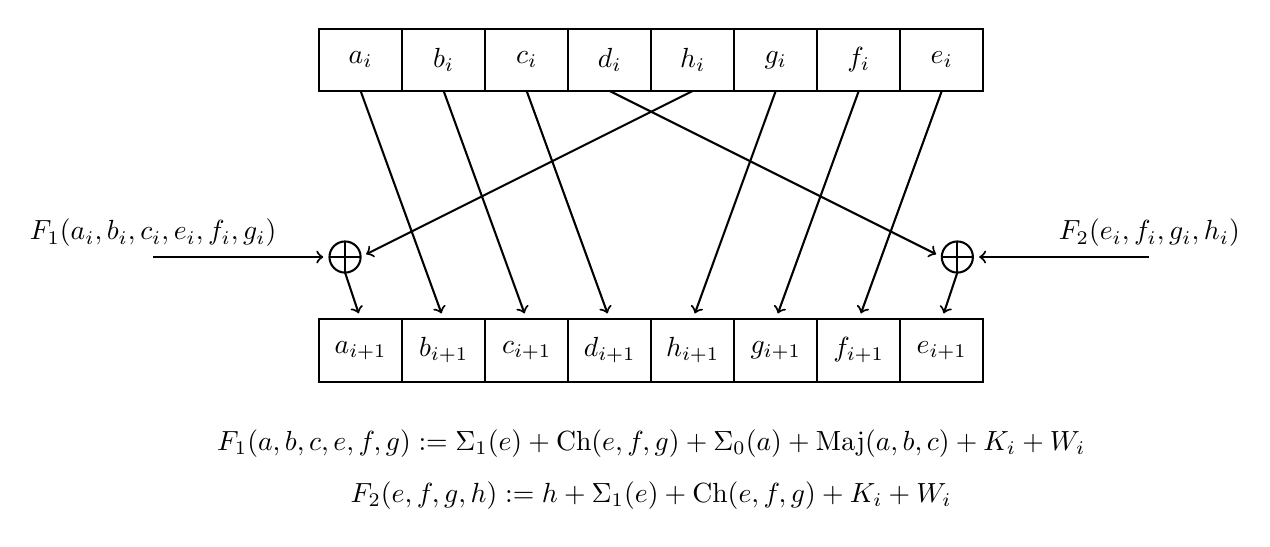
\begin{tikzpicture}[x=0.75pt,y=0.75pt,yscale=-1,xscale=1]

\draw   (100,0) -- (420,0) -- (420,30) -- (100,30) -- cycle ;
\draw   (100,140) -- (420,140) -- (420,170) -- (100,170) -- cycle ;
\draw    (140,0) -- (140,30) ;
\draw    (180,0) -- (180,30) ;
\draw    (220,0) -- (220,30) ;
\draw    (260,0) -- (260,30) ;
\draw    (300,0) -- (300,30) ;
\draw    (340,0) -- (340,30) ;
\draw    (380,0) -- (380,30) ;
\draw    (140,140) -- (140,170) ;
\draw    (180,140) -- (180,170) ;
\draw    (220,140) -- (220,170) ;
\draw    (260,140) -- (260,170) ;
\draw    (300,140) -- (300,170) ;
\draw    (340,140) -- (340,170) ;
\draw    (380,140) -- (380,170) ;

\draw  [->]  (120,30) -- (158.97,137.18) ;
\draw  [->]  (160,30) -- (198.97,137.18) ;
\draw  [->]  (200,30) -- (238.97,137.18) ;
\draw  [->]  (320,30) -- (281.03,137.18) ;
\draw  [->]  (360,30) -- (321.03,137.18) ;
\draw  [->]  (400,30) -- (361.03,137.18) ;
\draw  [->]  (240,30) -- (397.32,108.66) ;
\draw  [->]  (280,30) -- (122.68,108.66) ;
\draw  [->]  (112.5,117.5) -- (119.05,137.15) ;
\draw  [->]  (407.5,117.5) -- (400.95,137.15) ;
\draw  [->]  (20,110) -- (102,110) ;
\draw  [<-]  (418,110) -- (500,110) ;

% OR's
\draw   (105,110) .. controls (105,105.86) and (108.36,102.5) .. (112.5,102.5) .. controls (116.64,102.5) and (120,105.86) .. (120,110) .. controls (120,114.14) and (116.64,117.5) .. (112.5,117.5) .. controls (108.36,117.5) and (105,114.14) .. (105,110) -- cycle ;
\draw   (105,110) -- (120,110) ;
\draw   (112.5,102.5) -- (112.5,117.5) ;
\draw   (400,110) .. controls (400,105.86) and (403.36,102.5) .. (407.5,102.5) .. controls (411.64,102.5) and (415,105.86) .. (415,110) .. controls (415,114.14) and (411.64,117.5) .. (407.5,117.5) .. controls (403.36,117.5) and (400,114.14) .. (400,110) -- cycle ;
\draw   (400,110) -- (415,110) ;
\draw   (407.5,102.5) -- (407.5,117.5) ;


\draw (20,106.6) node [anchor=south] [inner sep=0.75pt]    {$F_{1}( a_{i} ,b_{i} ,c_{i} ,e_{i} ,f_{i} ,g_{i})$};
\draw (500,106.6) node [anchor=south] [inner sep=0.75pt]    {$F_{2}( e_{i} ,f_{i} ,g_{i} ,h_{i})$};
\draw (120,15) node    {$a_{i}$};
\draw (160,15) node    {$b_{i}$};
\draw (200,15) node    {$c_{i}$};
\draw (240,15) node    {$d_{i}$};
\draw (280,15) node    {$h_{i}$};
\draw (320,15) node    {$g_{i}$};
\draw (360,15) node    {$f_{i}$};
\draw (400,15) node    {$e_{i}$};
\draw (120,155) node    {$a_{i+1}$};
\draw (160,155) node    {$b_{i+1}$};
\draw (200,155) node    {$c_{i+1}$};
\draw (240,155) node    {$d_{i+1}$};
\draw (280,155) node    {$h_{i+1}$};
\draw (320,155) node    {$g_{i+1}$};
\draw (360,155) node    {$f_{i+1}$};
\draw (400,155) node    {$e_{i+1}$};
\draw (260,200) node    {$F_{1}( a,b,c,e,f,g) :=\Sigma _{1}( e) +\mathrm{Ch}( e,f,g) +\Sigma _{0}( a) +\mathrm{Maj}( a,b,c) +K_{i} +W_{i}$};
\draw (260,225) node    {$F_{2}( e,f,g,h) :=h+\Sigma _{1}( e) +\mathrm{Ch}( e,f,g) +K_{i} +W_{i}$};


\end{tikzpicture}
	\caption{SHA256分组密码的一轮}
	\label{fig:8-8}
\end{figure}
 
\subsection{其他 Merkle-Damg{\aa}rd 哈希函数}\label{subsec:8-6-1}

\begin{snote}[MD4和MD5。]
这两个密码学哈希函数都是由 Ron Rivest 在1990 到 1991 年设计的。它们两者都是 Merkle-Damg{\aa}rd 哈希函数,输出 $128$ 比特的摘要。它们非常相似,尽管 MD5 使用了比 MD4 更强的压缩函数。如表 \ref{tab:8-1} 所示,已经有算法能够有效地找到这两个哈希函数的碰撞。因此,它们都不应该再被使用在现实世界的系统之中。
\end{snote}

\begin{snote}[Whirpool。]
Whirlpool 由 Barreto 和 Rijmen 在 2000 年设计,并在 2004 年被采纳为 ISO/IEC 标准。Whirpool 是一个 Merkle-Damg{\aa}rd 哈希函数。它的压缩函数使用 Miyaguchi-Preneel 方法(见图 \ref{fig:8-7})和一个名为 $W$ 的分组密码。这个分组密码与 AES 非常相似,但是分组长度为 $512$ 比特。由此产生的哈希输出也是 $512$ 比特。
\end{snote}

\begin{snote}[其他算法。]
还有一些文献提出了许多其他的 Merkle-Damg{\aa}rd 哈希函数,比如 Tiger/192 和 RIPEMD-160。
\end{snote}
\section{案例研究:HMAC}\label{sec:8-7}

这一节,我们回过头来探讨之前的问题,即为长消息建立一个安全的 MAC。以 SHA256 为代表的 Merkle-Damg{\aa}rd 哈希函数已经被部署到了各种系统中。大多数密码学库都包含多种 Merkle-Damg{\aa}rd 函数的实现,而且这些实现往往都很快:通常情况下,用 SHA256 对一个很长的消息进行哈希要比用 AES 对相同的消息进行 CBC-MAC 要快得多。

当然,我们可以使用 \ref{sec:8-2} 节中所介绍的先哈希后MAC构造。回顾一下,在这个构造中,我们将一个安全的 MAC 系统 $\mathcal{I}=(S,V)$ 和一个抗碰撞哈希函数 $H$ 结合。由此产生的签名算法先使用 $H$ 对消息进行哈希,得到一个短的摘要 $H(m)$,然后使用 $S$ 对 $H(m)$ 进行签名,得到 MAC 标签 $t=S(k,H(m))$。正如我们在定理 \ref{theo:8-1} 中说明的,这样产生的构造是安全的。然而,这种构造并没有得到非常广泛的应用,这是为什么呢?

首先,正如我们在定理 \ref{theo:8-1} 之后所讨论的,如果我们可以找到 $H$ 的碰撞,先哈希后 MAC 构造就完全被破坏了。用于寻找碰撞的攻击,比如生日攻击(见 \ref{sec:8-3} 节),或者其他更复杂的攻击,都可以完全\emph{离线}进行,即不需要与任何系统用户交互。相对地,\emph{在线}攻击则需要对手和诚实的系统用户之间进行许多次交互。一般来说,我们认为离线攻击是特别危险的,因为对手可以在很长一段时间内投入巨大的计算资源:在对先哈希后 MAC 的攻击中,攻击者可以花上几个月的时间在许多机器上悄悄计算以找到 $H$ 上的碰撞,而不会引起任何怀疑。

另一个不直接使用先哈希后 MAC 构造的原因是,我们既需要一个哈希函数 $H$,也需要一个 MAC 系统 $\mathcal{I}$。因此,一个实现可能需要软件和/或硬件来执行哈希算法(比如 SHA256)和 MAC 算法(比如基于 AES 的 CBC-MAC)。在其他条件相同的情况下,如果能简单地只使用一种算法作为 MAC 的基础就更好了。

这就很自然地将我们导向这样一个问题:怎样基于一个\emph{无密钥}的 Merkle-Damg{\aa}rd 哈希函数(如 SHA256),以某种方式实现一个\emph{带密钥}的函数,它可以用作一个安全的 MAC,甚至是一个安全的 PRF?此外,我们希望能够在一个比抗碰撞更弱(至少是定性地)的假设下证明这个构造的安全性;特别地,这个构造应当不易受到针对底层压缩函数的离线碰撞查找攻击。

假设 $H$ 是一个由压缩函数 $h:\{0,1\}^n\times\{0,1\}^\ell\to\{0,1\}^n$ 构建的 Merkle-Damg{\aa}rd 哈希。我们可以想到下面几种简单的方法:
\begin{description}
	\item [前缀密钥:] $F_\mathrm{pre}(k,M):=H(k\,\Vert\,M)$。这种思路完全是不安全的,因为存在这样的一种\emph{扩展攻击}:给定 $F\mathrm{pre}(k,M)$,我们很容易为任意的 $M'$ 计算出 $F_\mathrm{pre}(k,M\,\Vert\,\mathrm{PB}\,\Vert\,M')$。这里的 $\mathrm{PB}$ 是消息 $k\,\Vert\,M$ 的 Merkle-Damg{\aa}rd 填充分组。如果排除这种扩展攻击,那么在合理的假设条件下,这个构造是安全的(见练习 \ref{exer:8-18})。
	\item [后缀密钥:] $F_\mathrm{post}(k,M):=H(M\,\Vert\,k)$。这种构造有点类似于先哈希后 MAC 构造,并且依赖于 $h$ 的抗碰撞性。事实上,该构造很容易受到离线碰撞查找攻击:假设我们能找到两个不同的 $\ell$ 比特序列 $M_0$ 和 $M_1$ 满足 $h(\mathrm{IV},M_0)=h(\mathrm{IV},M_1)$,我们就有 $F_\mathrm{post}(k,M_0)=F_\mathrm{post}(k,M_1)$。因此,这个构造也无法解决我们的问题。然而,在恰当的假设条件下(当然,也包括对 $h$ 抗碰撞性的假设),我们仍然能够得到该构造的安全证明(见练习 \ref{exer:8-19})。
	\item [密钥包裹:] $F_\mathrm{env}(k,M):=H(k\,\Vert\,M\,\Vert\,k)$。在对 $h$ 合理的伪随机性假设以及某种格式假设($k$是一个 $\ell$ 比特序列,$M$ 被填充为一个长度为 $\ell$ 的整数倍的序列)下,可以证明该构造是一个安全的PRF。见练习 \ref{exer:8-17}。
	\item [双层密钥嵌套:] $F_\mathrm{nest}((k_1,k_2),M):=H(k_2\,\Vert\,H(k_1\,\Vert\,M))$。在对 $h$ 合理的伪随机性假设和种格式假设($k_1$ 和 $k2$ 都是 $\ell$ 比特序列)下,该构造也可以被证明是一个安全的 PRF。
\end{description}

双层密钥嵌套与一个被称为 HMAC 的经典 MAC 构造密切相关。HMAC 是互联网上应用最广泛的 MAC。它被用于 SSL、TLS、IPsec、SSH 和许多其他的安全协议中。TLS 和 IPsec 在会话设置过程中使用 HMAC 来生成会话密钥。下面,我们分析双层密钥嵌套的安全性,然后讨论它与 HMAC 的关系。

\begin{figure}
	\centering
	\tikzset{every picture/.style={line width=0.75pt}}

\begin{tikzpicture}[x=0.75pt,y=0.75pt,yscale=-1,xscale=1]

\draw  [fill={rgb, 255:red, 255; green, 255; blue, 255 }  ,fill opacity=1 ][line width=1.2] [general shadow={fill=black,shadow xshift=2.25pt,shadow yshift=-2.25pt}] (110,85) -- (110,110) -- (60,110) -- (60,70) -- cycle ;
\draw  [fill={rgb, 255:red, 255; green, 255; blue, 255 }  ,fill opacity=1 ][line width=1.2] [general shadow={fill=black,shadow xshift=2.25pt,shadow yshift=-2.25pt}] (210,85) -- (210,110) -- (160,110) -- (160,70) -- cycle ;
\draw  [fill={rgb, 255:red, 255; green, 255; blue, 255 }  ,fill opacity=1 ][line width=1.2] [general shadow={fill=black,shadow xshift=2.25pt,shadow yshift=-2.25pt}] (380,85) -- (380,110) -- (330,110) -- (330,70) -- cycle ;
\draw  [fill={rgb, 255:red, 255; green, 255; blue, 255 }  ,fill opacity=1 ][line width=1.2] [general shadow={fill=black,shadow xshift=2.25pt,shadow yshift=-2.25pt}] (380,225) -- (380,250) -- (330,250) -- (330,210) -- cycle ;
\draw  [fill={rgb, 255:red, 255; green, 255; blue, 255 }  ,fill opacity=1 ][line width=1.2] [general shadow={fill=black,shadow xshift=2.25pt,shadow yshift=-2.25pt}] (480,225) -- (480,250) -- (430,250) -- (430,210) -- cycle ;

\draw  [line width=1.2]  (10,10) -- (80,10) -- (80,30) -- (10,30) -- cycle ;
\draw  [line width=1.2]  (110,10) -- (180,10) -- (180,30) -- (110,30) -- cycle ;
\draw  [line width=1.2]  (280,10) -- (350,10) -- (350,30) -- (280,30) -- cycle ;
\draw  [line width=1.2]  (280,150) -- (350,150) -- (350,170) -- (280,170) -- cycle ;
\draw  [line width=1.2]  (380,150) -- (450,150) -- (450,170) -- (380,170) -- cycle ;

\draw    (210,100) -- (250,100) ;
\draw  [->]  (10,100) -- (59,100) ;
\draw  [->]  (110,100) -- (159,100) ;
\draw  [->]  (290,100) -- (329,100) ;
\draw  [->]  (480,240) -- (520,240) ;
\draw  [->]  (280,240) -- (329,240) ;
\draw  [->]  (380,240) -- (429,240) ;

\draw  [->]  (45,30) -- (45,80) -- (59,80) ;
\draw  [->]  (145,30) -- (145,80) -- (159,80) ;
\draw  [->]  (315,30) -- (315,80) -- (329,80) ;
\draw  [->]  (315,170) -- (315,220) -- (329,220) ;
\draw  [->]  (415,170) -- (415,220) -- (429,220) ;
\draw  [->]  (380,100) -- (415,100) -- (415,149) ;

\draw   (64.95,80) -- (59.95,83.5) -- (59.95,76.5) -- cycle ;
\draw   (165,100) -- (160,103.5) -- (160,96.5) -- cycle ;
\draw   (335,100) -- (330,103.5) -- (330,96.5) -- cycle ;
\draw   (435,240) -- (430,243.5) -- (430,236.5) -- cycle ;
\draw   (334.95,220) -- (329.95,223.5) -- (329.95,216.5) -- cycle ;

\draw  [dash pattern={on 4.5pt off 4.5pt}][line width=0.75]  (95,0) -- (95,60) -- (120,60) -- (120,120) -- (0,120) -- (0,0) -- cycle ;
\draw  [dash pattern={on 4.5pt off 4.5pt}][line width=0.75]  (365,140) -- (365,200) -- (390,200) -- (390,260) -- (270,260) -- (270,140) -- cycle ;
\draw  [dash pattern={on 0.84pt off 2.51pt}]  (250,100) -- (290,100) ;


\draw (85,95) node  [font=\small]  {$h$};
\draw (185,95) node  [font=\small]  {$h$};
\draw (355,95) node  [font=\small]  {$h$};
\draw (45,20) node  [font=\small]  {$k_{1}$};
\draw (145,20) node  [font=\small]  {$m_{1}$};
\draw (315,20) node  [font=\small]  {$m_{s} \ \| \ \mathrm{PB}_{\mathrm{i}}$};
\draw (12,96.6) node [anchor=south west] [inner sep=0.75pt]  [font=\small]  {$\mathrm{IV}$};
\draw (135,96.6) node [anchor=south] [inner sep=0.75pt]  [font=\small]  {$k'_{1}$};
\draw (230,20) node    {$\cdots $};
\draw (355,235) node  [font=\small]  {$h$};
\draw (455,235) node  [font=\small]  {$h$};
\draw (315,160) node  [font=\small]  {$k_{2}$};
\draw (405,236.6) node [anchor=south] [inner sep=0.75pt]  [font=\small]  {$k'_{2}$};
\draw (282,236.6) node [anchor=south west] [inner sep=0.75pt]  [font=\small]  {$\mathrm{IV}$};
\draw (415,160) node  [font=\small]  {$t\ \| \ \mathrm{PB}_{\mathrm{o}}$};
\draw (397.5,96.62) node [anchor=south] [inner sep=0.75pt]  [font=\small]  {$t$};

\end{tikzpicture}
	\caption{双层密钥嵌套}
	\label{fig:8-9}
\end{figure}

\subsection{双层密钥嵌套的安全性}\label{subsec:8-7-1}

现在我们证明,在对 $h$ 进行适当的伪随机性假设的情况下,双层密钥嵌套确实是一个安全的 PRF。首先,考虑到 $H$ 是由 $h$ 建立的 Merkle-Damg{\aa}rd 哈希,我们试着``拆开" $F_\mathrm{nest}((k_1,k_2),M)$ 的定义,见图 \ref{fig:8-9}。读者应该仔细研究这张图。我们假设密钥 $k_1$ 和 $k_2$ 都是 $\ell$ 比特的序列,所以它们各自占据一个完整的消息分组。$H$ 内圈计算的输入是填充后的序列 $k_1\,\Vert\,M\,\Vert\,\mathrm{PB}_\mathrm{i}$,它会被拆分为一系列长为 $\ell$ 比特的分组。$H$ 内圈计算的输出是一个 $n$ 比特序列 $t$。$H$ 外圈计算的输入是填充后的序列 $k_2\,\Vert\,t\,\Vert\,\mathrm{PB}_\mathrm{o}$。我们假设 $n$ 远小于 $\ell$,所以 $t\,\Vert\,\mathrm{PB}_\mathrm{o}$ 就是一个单独的 $\ell$ 比特分组,如图所示。

下面介绍我们所需的伪随机性假设。我们定义下面两个由 $h$ 派生的 PRF $h_\mathrm{bot}$ 和 $h_\mathrm{top}$:
\begin{equation}\label{eq:8-6}
h_\mathrm{bot}(k,m):=h(k,m),
\qquad
h_\mathrm{top}(k,m):=h(m,k)
\end{equation}
对于 PRF $h_\mathrm{bot}$,PRF 密钥 $k$ 被视作 $h$ 的第一个输入,即 $n$ 比特的链式变量输入,它是图 \ref{fig:8-9} 中 $h$ 盒的\emph{底部}输入。对于 PRF $h_\mathrm{top}$,PRF密钥 $k$ 被视为 $h$ 的第二个输入,即 $\ell$ 比特的消息分组输入,它是图中 $h$ 盒的\emph{顶部}输入。为了使该图更容易理解,我们用一个 $\triangleright$ 符号来标记 $h$ 盒的输入,用于指示被视作 PRF 密钥的那一个输入。事实上,读者很容易注意到,我们将虚线框内的两个 $h$ 计算视作 PRF $h_\mathrm{top}$ 的计算,因此,图中标有 $k_1'$ 和 $k_2'$ 的值由 $k_1'\leftarrow h_\mathrm{top}(k_1,\mathrm{IV})$ 和 $k_1'\leftarrow h_\mathrm{top}(k_2,\mathrm{IV})$ 计算而来。图中所有其他的 $h$ 计算都被视作对 $h_\mathrm{bot}$ 的计算。

我们的假设是,$h_\mathrm{bot}$ 和 $h_\mathrm{top}$ 都是安全的 PRF。稍后,我们将使用理想密码模型对 Davies-Meyer 压缩函数证明这一假设(见 \ref{subsec:8-7-3} 小节)。

现在,我们先对以下结论给出一个简单的证明:
\begin{quote}
\emph{如果 $h_\mathrm{bot}$ 和 $h_\mathrm{top}$ 都是安全的 PRF,那么双层密钥嵌套也是安全的。}
\end{quote}

第一个观察是,密钥 $k_1$ 和 $k_2$ 只被用于派生 $k_1'$ 和 $k_2'$,即 $k_1'=h_\mathrm{top}(k_1,\mathrm{IV})$,$k_2'=h_\mathrm{top}(k_2,\mathrm{IV})$。假设 $h_\mathrm{top}$ 是一个安全的 PRF,就意味着在 PRF 攻击游戏中,我们可以有效地用真随机的 $n$ 比特序列替换 $k_1'$ 和 $k_2'$。图 \ref{fig:8-10} 展示了由此产生的构造。这里,我们所做的就是去掉图 \ref{fig:8-9} 中所有虚线框内的元素。这个新构造中的函数将两个密钥 $k_1'$ 和 $k_2'$ 以及一条消息 $M$ 作为输入。根据以上观察,我们只需证明图 \ref{fig:8-10} 中的构造是一个安全的 PRF 即可。

\begin{figure}
	\centering
	\tikzset{every picture/.style={line width=0.75pt}}

\begin{tikzpicture}[x=0.75pt,y=0.75pt,yscale=-1,xscale=1]


\draw  [fill={rgb, 255:red, 255; green, 255; blue, 255 }  ,fill opacity=1 ][line width=1.2] [general shadow={fill=black,shadow xshift=2.25pt,shadow yshift=-2.25pt}] (100,85) -- (100,110) -- (50,110) -- (50,70) -- cycle ;
\draw  [fill={rgb, 255:red, 255; green, 255; blue, 255 }  ,fill opacity=1 ][line width=1.2] [general shadow={fill=black,shadow xshift=2.25pt,shadow yshift=-2.25pt}] (270,85) -- (270,110) -- (220,110) -- (220,70) -- cycle ;
\draw  [fill={rgb, 255:red, 255; green, 255; blue, 255 }  ,fill opacity=1 ][line width=1.2] [general shadow={fill=black,shadow xshift=2.25pt,shadow yshift=-2.25pt}] (370,225) -- (370,250) -- (320,250) -- (320,210) -- cycle ;

\draw  [line width=1.2]  (0,10) -- (70,10) -- (70,30) -- (0,30) -- cycle ;
\draw  [line width=1.2]  (170,10) -- (240,10) -- (240,30) -- (170,30) -- cycle ;
\draw  [line width=1.2]  (270,150) -- (340,150) -- (340,170) -- (270,170) -- cycle ;

\draw    (100,100) -- (140,100) ;
\draw  [->]  (0,100) -- (49,100) ;
\draw  [->]  (180,100) -- (219,100) ;
\draw  [->]  (270,240) -- (319,240) ;
\draw  [->]  (370,240) -- (410,240) ;
\draw  [->]  (35,30) -- (35,80) -- (49,80) ;
\draw  [->]  (205,30) -- (205,80) -- (219,80) ;
\draw  [->]  (270,100.04) -- (305,100) -- (305,149) ;
\draw  [->]  (305,170) -- (305,220) -- (319,220) ;

\draw   (55,100) -- (50,103.5) -- (50,96.5) -- cycle ;
\draw   (225,100) -- (220,103.5) -- (220,96.5) -- cycle ;
\draw   (325,240) -- (320,243.5) -- (320,236.5) -- cycle ;

\draw  [dash pattern={on 0.84pt off 2.51pt}]  (140,100) -- (180,100) ;


\draw (75,95) node  [font=\small]  {$h$};
\draw (245,95) node  [font=\small]  {$h$};
\draw (35,20) node  [font=\small]  {$m_{1}$};
\draw (205,20) node  [font=\small]  {$m_{s} \ \| \ \mathrm{PB}_{\mathrm{i}}$};
\draw (2,96.6) node [anchor=south west] [inner sep=0.75pt]  [font=\small]  {$k'_{1}$};
\draw (120,20) node    {$\cdots $};
\draw (345,235) node  [font=\small]  {$h$};
\draw (272,236.6) node [anchor=south west] [inner sep=0.75pt]  [font=\small]  {$k'_{2}$};
\draw (305,160) node  [font=\small]  {$t\ \| \ \mathrm{PB}_{\mathrm{o}}$};
\draw (287.5,96.62) node [anchor=south] [inner sep=0.75pt]  [font=\small]  {$t$};


\end{tikzpicture}
	\caption{NMAC 的一个按比特版本}
	\label{fig:8-10}
\end{figure}

希望即使不看标题,读者也能认出图 \ref{fig:8-10} 中的构造正是将我们在 \ref{subsec:6-5-1} 小节中介绍的 NMAC 应用在 $h_\mathrm{bot}$ 上的结果(特别是,请注意图 \ref{fig:6-5-b})。实际上,图 \ref{fig:8-10} 中的构造是 NMAC 的一个按比特版本,我们可以借由填充从按分组版本中得到它(如 \ref{sec:6-8} 节所述)。因此,在假设 $h_\mathrm{bot}$ 是一个安全 PRF 的情况下,双层密钥嵌套的安全性可以直接由 NMAC 安全定理(定理 \ref{theo:6-7})得到。

\subsection{HMAC 标准}\label{subsec:8-7-2}

HMAC 标准与双层密钥嵌套(图 \ref{fig:8-9})基本相同,但有一个重要的区别:在 HMAC 中,密钥 $k_1$ 和 $k_2$ 并不相互独立,而是以一种有点特别的方式由单一密钥 $k$ 派生而来。

为了更详细地描述这一点,我们首先观察到,HMAC 本身在某种程度上是面向字节的,所以所有序列都是字节序列。底层 Merkle-Damg{\aa}rd 哈希的消息分组被假定为 $B$ 字节(而不是 $\ell$ 比特)。HMAC 的密钥 $k$ 是一个任意长度的序列。为了得到密钥 $k_1$ 和 $k_2$(都是长为 $B$字节的序列),我们首先迫使 $k$ 的长度正好是 $B$ 字节:如果 $k$ 的长度小于或等于 $B$ 字节,我们就用零字节来填充它;否则,我们就用零字节填充的 $H(k)$ 来代替它。然后,我们计算:
\[
k_1\leftarrow k\oplus\mathsf{ipad},
\qquad
k_2\leftarrow k\oplus\mathsf{opad}
\]
其中,$\mathsf{ipad}$ 和 $\mathsf{opad}$(`i' 和 `o' 分别代表``内部" 和 ``外部")都是 $B$ 字节的常量序列,定义如下:
\[
\begin{aligned}
& \mathsf{ipad}:=\texttt{0x36}\;\text{\emph{重复}}\;B\;\text{\emph{次}}\\
& \mathsf{opad}:=\texttt{0x5C}\;\text{\emph{重复}}\;B\;\text{\emph{次}}
\end{aligned}
\]

使用哈希函数 $H$ 实现的 HMAC 被称作 HMAC-$H$。在实践中最常用的 HMAC 是 HMAC-SHA1 和 HMAC-SHA256。HMAC 标准还允许对 HMAC 的输出进行截短。例如,当把 SHA1 的输出截短到 $80$ 比特时,相应的 HMAC 函数就被称作 HMAC-SHA1-80。举例来说,TLS 1.0 的实现就被要求能够支持 HMAC-SHA1-96。

\begin{snote}[HMAC 的安全性。]
由于密钥 $k_1'$ 和 $k_2'$ 是相关的(它们的异或就等于 $\mathsf{opad}\oplus\mathsf{ipad}$),我们为双层密钥嵌套所提出的安全证明就不再能够适用:在所述假设下,我们不能证明派生出的密钥 $k_1'$ 与 $k_2'$ 和随机元是不可区分的。一个解决方案是对压缩函数 $h$ 做一个更强的假设——我们需要假设 $h_\mathrm{top}$ 在关联密钥攻击下仍然是一个 PRF(如 Bellare 和 Kohno 的定义)。如果 $h$ 本身是一个 Davies-Meyer 压缩函数,那么在理想密码模型下,这个更强的假设仍能得到证明。
\end{snote}

\subsection{Davies-Meyer 在理想密码模型下是安全的 PRF}\label{subsec:8-7-3}

剩下的工作就是证明我们的假设,即式 \ref{eq:8-6} 中由 $h$ 派生的 $h_\mathrm{bot}$ 和 $h_\mathrm{top}$ 都是安全的 PRF。假设压缩函数 $h$ 是一个 Davies-Meyer 函数,即 $h(x,y):=E(y,x)\oplus x$,其中,$\mathcal{E}=(E,D)$ 是某个分组密码。那么:
\begin{itemize}
	\item $h_\mathrm{bot}(k,m):=h(k,m)=E(m,k)\oplus k$ 是一个定义在 $(\mathcal{X},\mathcal{K},\mathcal{X})$ 上的 PRF,并且
	\item $h_\mathrm{top}(k,m):=h(m,k)=E(k,m)\oplus m$ 是一个定义在 $(\mathcal{K},\mathcal{X},\mathcal{X})$ 上的 PRF。
\end{itemize}
当 $\mathcal{E}$ 是一个安全的分组密码时,$h_\mathrm{top}$ 显然是一个安全的 PRF(见练习 \ref{exer:4-1} 的 (c) 部分)。但 $h_\mathrm{bot}$ 是一个安全 PRF 的事实有点令人惊讶——作为 $h_\mathrm{bot}$ 输入的消息 $m$ 被用作 $E$ 的密钥。因此,即使 $\mathcal{E}$ 是一个安全的分组密码,$h_\mathrm{bot}$ 也无法提供安全性保证。尽管如此,我们仍然可以证明 $h_\mathrm{bot}$ 是一个安全的 PRF,但这需要在理想密码模型下。仅仅假设 $\mathcal{E}$ 是一个安全分组密码是不充分的。

如有必要,读者可以回顾 \ref{sec:4-7} 节中介绍的理想密码模型的基本概念。我们在本章的稍早部分也使用了理想密码模型(见 \ref{subsec:8-5-3} 小节)。

在理想密码模型中,我们启发式地将一个定义在 $(\mathcal{K},\mathcal{X})$ 上的分组密码 $\mathcal{E}=(E,D)$ 建模为一个随机置换族 $\{\Pi_\mathpzc{k}\}_{\mathpzc{k}\in\mathcal{K}}$。我们改编 PRF 攻击游戏 \ref{game:4-2},让它适用于理想密码模型。挑战者除了应答标准查询外,还要应答 $\Pi$-查询和 $\Pi^{-1}$-查询:一个$\Pi$-查询是一个数对 $(\mathpzc{k},\mathpzc{a})$,挑战者以 $\mathpzc{b}:=\Pi_\mathpzc{k}(\mathpzc{a})$ 作为应答。$\Pi^{-1}$-查询是一个数对 $(\mathpzc{k},\mathpzc{b})$,挑战者以 $\mathpzc{a}:=\Pi_\mathpzc{k}^{-1}(\mathpzc{b})$ 作为应答。对于一个标准查询 $m$,挑战者以 $v:=f(m)$ 作为应答:在攻击游戏的实验 $0$ 中,$f$ 是 $F(k,\cdot)$,其中的 $F$ 是一个 PRF,$k$ 是一个随机选出的密钥;在实验 $1$ 中,$f$ 是一个真随机函数。此外,在实验 $0$ 中,用于评估 $F$ 的随机置换就是在构建 $F$ 时用作 $E$ 和 $D$ 的置换。对于我们的 PRF,我们有 $h_\mathrm{bot}(k,m)=E(m,k)\oplus k=\Pi_m(k)\oplus k$。

对于对手 $\mathcal{A}$,我们将它在修改后的 PRF 攻击游戏中的优势定义为 $\mathrm{PRF}^\mathrm{ic}\mathsf{adv}[\mathcal{A},F]$,理想密码模型上的安全性意味着,该优势对于所有有效对手来说都可忽略不计。

\begin{theorem}[$h_\mathrm{bot}$ 的安全性]\label{theo:8-5}
令 $\mathcal{E}=(E,D)$ 是一个定义在 $(\mathcal{K},\mathcal{X})$ 上的分组密码,其中 $|\mathcal{X}|$ 是大的。那么在理想密码模型下,$h_\mathrm{bot}(k,m):=E(m,k)\oplus k$ 是一个安全的 PRF。
\begin{quote}
特别地,对于每个攻击 $h_\mathrm{bot}$ 的 PRF 对手 $\mathcal{A}$,如果它最多只能发起 $Q_\mathrm{ic}$ 次理想密码查询,我们就有:
\end{quote}
\[
\mathrm{PRF}^\mathrm{ic}\mathsf{adv}[\mathcal{A},h_\mathrm{bot}]\leq\frac{2Q_\mathrm{ic}}{|\mathcal{X}|}
\]
\end{theorem}

该定理中的上界是相当严格的,因为对密钥进行暴力搜索能非常接近该约束。

\begin{proof}
该证明与对 Evan-Mansour/$\mathcal{E}$X 构造的分析如出一辙(见 \ref{subsec:4-7-4} 小节的定理 \ref{theo:4-14}),特别是,该证明会用到领域分离定理(见第 \ref{subsec:4-7-4} 小节的定理 \ref{theo:4-15})。

令 $\mathcal{A}$ 是一个定理声明中的对手。记 $p_b$ 为 $\mathcal{A}$ 在攻击游戏 \ref{game:4-2} 的实验 $b$ 中输出 $1$ 的概率,其中 $b=0,1$。所以,根据定义,我们有:
\begin{equation}\label{eq:8-7}
\mathrm{PRF}^\mathrm{ic}\mathsf{adv}[\mathcal{A},h_\mathrm{bot}]=|p_0-p_1|
\end{equation}

下面,我们构造一个有两个游戏组成的游戏序列,并应用领域分离引理来证明该定理。

\vspace{5pt}

\noindent\textbf{游戏 $\mathbf{0}$。}
该游戏对应于理想密码模型下 PRF 攻击游戏的实验 $0$。我们可以将挑战者的逻辑表述如下:

\vspace{5pt}

\hspace*{5pt} 初始化:\\
\hspace*{50pt} 对于每个 $\mathpzc{k}\in\mathcal{K}$,随机选取 $\Pi_\mathpzc{k}\overset{\rm R}\leftarrow\mathrm{Perms}[\mathcal{X}]$\\
\hspace*{50pt} 随机选取 $k\overset{\rm R}\leftarrow\mathcal{X}$

\vspace{5pt}

\hspace*{5pt} 标准 $h_\mathrm{bot}$-查询 $m$:\\
\hspace*{26pt} 1.\qquad 令 $c\leftarrow\Pi_m(k)$\\
\hspace*{26pt} 2.\qquad 令 $v\leftarrow c\oplus k$\\
\hspace*{26pt} 3.\qquad 返回 $v$

\vspace{5pt}

游戏 $0$ 中的挑战者\emph{完全按照定理 \ref{theo:4-14} 的证明中的游戏 $0$} 来处理理想密码查询:

\vspace{5pt}

\hspace*{5pt} 理想密码 $\Pi$-查询 $\mathpzc{k},\mathpzc{a}$:\\
\hspace*{26pt} 1.\qquad 令 $\mathpzc{b}\leftarrow\Pi_\mathpzc{k}(\mathpzc{a})$\\
\hspace*{26pt} 2.\qquad 返回 $\mathpzc{b}$

\vspace{5pt}

\hspace*{5pt} 理想密码 $\Pi^{-1}$-查询 $\mathpzc{k},\mathpzc{b}$:\\
\hspace*{26pt} 1.\qquad 令 $\mathpzc{a}\leftarrow\Pi_\mathpzc{k}^{-1}(\mathpzc{b})$\\
\hspace*{26pt} 2.\qquad 返回 $\mathpzc{a}$

\vspace{5pt}

令 $W_0$ 为 $\mathcal{A}$ 在游戏 $0$ 结束时输出 $1$ 的事件。从构造上看,显然有:
\begin{equation}\label{eq:8-8}
\Pr[W_0]=p_0
\end{equation}

\noindent\textbf{游戏 $\mathbf{1}$。}
同定理 \ref{theo:4-14} 的证明一样,我们``凭空"宣布,标准查询和理想密码查询都是使用相互独立的随机置换处理的。下面是具体的逻辑,与游戏 $0$ 不同的部分被高亮强调:

\vspace{5pt}

\hspace*{5pt} 初始化:\\
\hspace*{50pt} 对于每个 $\mathpzc{k}\in\mathcal{K}$,随机选取 \colorbox{gray!50}{$\Pi_{\mathrm{std},\mathpzc{k}}\overset{\rm R}\leftarrow\mathrm{Perms}[\mathcal{X}]$ 和 $\Pi_{\mathrm{ic},\mathpzc{k}}\overset{\rm R}\leftarrow\mathrm{Perms}[\mathcal{X}]$}\\
\hspace*{50pt} 随机选取 $k\overset{\rm R}\leftarrow\mathcal{X}$

\vspace{5pt}

\hspace*{5pt} 标准 $h_\mathrm{bot}$-查询 $m$:\\
\hspace*{26pt} 1.\qquad 令 $c\leftarrow$\colorbox{gray!50}{$\Pi_{\mathrm{std},m}(k)$}
\quad//\quad\emph{将 $k$ 添加到 $\Pi_{\mathrm{std},m}$ 的采样领域,将 $c$ 添加到 $\Pi_{\mathrm{std},m}$ 的采样范围}\\
\hspace*{26pt} 2.\qquad 令 $v\leftarrow c\oplus k$\\
\hspace*{26pt} 3.\qquad 返回 $v$

\vspace{5pt}

游戏 $1$ 中的挑战者\emph{完全按照定理 \ref{theo:4-14} 的证明中的游戏 $1$} 来处理理想密码查询:

\vspace{5pt}

\hspace*{5pt} 理想密码 $\Pi$-查询 $\mathpzc{k},\mathpzc{a}$:\\
\hspace*{26pt} 1.\qquad 令 $\mathpzc{b}\leftarrow$\colorbox{gray!50}{$\Pi_{\mathrm{ic},\mathpzc{k}}(\mathpzc{a})$}
\;\;\quad//\quad\emph{将 $\mathpzc{a}$ 添加到 $\Pi_{\mathrm{ic},\mathpzc{k}}$ 的采样领域,将 $\mathpzc{b}$ 添加到 $\Pi_{\mathrm{ic},\mathpzc{k}}$ 的采样范围}\\
\hspace*{26pt} 2.\qquad 返回 $\mathpzc{b}$

\vspace{5pt}

\hspace*{5pt} 理想密码 $\Pi^{-1}$-查询 $\mathpzc{k},\mathpzc{b}$:\\
\hspace*{26pt} 1.\qquad 令 $\mathpzc{a}\leftarrow$\colorbox{gray!50}{$\Pi_{\mathrm{ic},\mathpzc{k}}^{-1}(\mathpzc{b})$}
\;\;\quad//\quad\emph{将 $\mathpzc{a}$ 添加到 $\Pi_{\mathrm{ic},\mathpzc{k}}$ 的采样领域,将 $\mathpzc{b}$ 添加到 $\Pi_{\mathrm{ic},\mathpzc{k}}$ 的采样范围}\\
\hspace*{26pt} 2.\qquad 返回 $\mathpzc{a}$

\vspace{5pt}

令 $W_1$ 为 $\mathcal{A}$ 在游戏 $1$ 结束时输出 $1$ 的事件。考虑游戏 $1$ 中一次标准查询的一个输入/输出对 $(m,v)$。注意到,$k$ 是唯一一个被添加到 $\Pi_{\mathrm{std},m}(k)$ 的采样领域中的项,而 $c=v\oplus k$ 是唯一一个被添加到 $\Pi_{\mathrm{std},m}(k)$ 的采样范围中的项。特别是,$c$ 是随机生成的,而 $k$ 始终保持完美隐藏(即与对手的观察无关)。

因此,从对手的角度来看,标准查询的行为与随机函数相同,而理想密码查询的行为与一个\emph{独立的}理想密码的理想密码查询相同。特别地,我们有:
\begin{equation}\label{eq:8-9}
\Pr[W_1]=p_1
\end{equation}

最后,我们使用领域分离引理来分析 $|\Pr[W_0]-\Pr[W_1]|$。领域分离失败事件 $Z$ 是指在游戏 $1$ 中,$\Pi_{\mathrm{std},m}$ 的一个采样领域与 $\Pi_{\mathrm{ic},\mathpzc{k}}$ 的一个采样领域重叠,或者 $\Pi_{\mathrm{std},m}$ 的一个采样范围与 $\Pi_{\mathrm{ic},\mathpzc{k}}$ 的一个采样范围重叠的事件。领域分离引理告诉我们,有:
\begin{equation}\label{eq:8-10}
|\Pr[W_0]-\Pr[W_1]|\leq\Pr[Z]
\end{equation}

如果事件 $Z$ 发生,那么对于某个对应于一个理想密码查询的输入/输出三元组 $(\mathpzc{k},\mathpzc{a},\mathpzc{b})$,$\mathpzc{k}=m$ 是一个输出为 $v$ 的标准查询的输入,并且:
\begin{enumerate}[(i)]
	\item $\mathpzc{a}=k$,或者
	\item $\mathpzc{b}=v\oplus k$
\end{enumerate}
成立。对于任何固定三元组 $(\mathpzc{k},\mathpzc{a},\mathpzc{b})$,根据 $k$ 的独立性,条件 (i) 和 (ii) 成立的概率都是 $1/|\mathcal{X}|$,因此,根据联合约束,我们有:
\begin{equation}\label{eq:8-11}
\Pr[Z]\leq\frac{2Q_\mathrm{ic}}{|\mathcal{X}|}
\end{equation}

于是,根据式 \ref{eq:8-7},\ref{eq:8-8},\ref{eq:8-9},\ref{eq:8-10} 和 \ref{eq:8-11},该定理成立。
\end{proof} 
\section{海绵构造与 SHA3}\label{sec:8-8}
\section{Merkle树:证明哈希列表的属性}\label{sec:8-9}

既然我们已经了解了如何构建抗碰撞函数,那么,让我们看看它们在数据完整性方面都有哪些应用。考虑一个大的可执行文件,它以 $\ell$ 比特的短分组 $x_1,\dots,x_n$ 的形式被存储在磁盘上。操作系统每次加载和运行这个可执行文件之前,都需要验证其内容没有被篡改。在本章的前言部分,我们讨论了如何在只读存储器中保存整个文件的短哈希值\footnotemark[3]。每当要运行文件时,系统首先重新计算文件的哈希值,并验证它是否与存储中的哈希值一致。我们说,抗碰撞哈希能确保对手无法篡改文件而不被发现。问题是,对于一个大文件来说,计算整个文件的哈希可能需要相当长的时间,而这将大大增加启动可执行文件的耗时。

\footnotetext[3]{回顾一下,只读存储器可以被对手读取,但是不能被修改。它可以被实现为一个独立的系统,向任何要求获得数据的人提供数据。或者,更简单地说,它可以通过使用数字签名方案(见第\ref{chap:13}章)签署数据来实现,并离线存储签名密钥。}

可以改进这一点吗?为了开始运行可执行文件,系统只需验证第一个分组 $x_1$。当执行流转移到其他分组时,系统再去验证相应的分组,以此类推。换句话说,与其一次性验证整个文件,不如让系统在加载相关内容时再去验证它。对于这种设计思路,一个可行的方案是预先计算所有分组 $x_1,\dots,x_n$ 的哈希值,并将产生的 $n$ 个哈希值存储在只读存储器中。这样,验证每个分组都很容易,但问题是,存储这 $n$ 个哈希值需要占用大量的只读空间。幸运的是,我们有一个更好的解决方案。

\begin{snote}[Merkle 树。]
为了重述这个的问题,我们有一个包含 $n$ 项的向量 $T:=(x_1,\dots,x_n)\in\mathcal{X}^n$,我们希望计算这个向量的一个短哈希值 $y$。之后,我们可能会被给予哈希值 $y$ 和数对 $(i,x)$,其中 $1\leq i\leq n$。我们需要验证 $x$ 是否是 $T$ 中的第 $i$ 项。

这个问题的解决方案是一个聪明的数据结构,称为 \textbf{Merkle 树},如图 \ref{fig:8-12} 所示。由此产生的哈希函数 $H$ 被称为 \textbf{Merkle 树哈希 (Merkle tree hash)}。

\begin{figure}
	\centering
	

\tikzset{every picture/.style={line width=0.75pt}} %set default line width to 0.75pt        

\begin{tikzpicture}[x=0.75pt,y=0.75pt,yscale=-1,xscale=1]
%uncomment if require: \path (0,249); %set diagram left start at 0, and has height of 249

%Straight Lines [id:da702920327532164] 
\draw [fill={rgb, 255:red, 255; green, 255; blue, 255 }  ,fill opacity=1 ][line width=0.75]    (222.4,54.69) -- (115,90) ;
\draw [shift={(225.25,53.76)}, rotate = 161.8] [fill={rgb, 255:red, 0; green, 0; blue, 0 }  ][line width=0.08]  [draw opacity=0] (7.14,-3.43) -- (0,0) -- (7.14,3.43) -- cycle    ;
%Straight Lines [id:da3073933646499085] 
\draw [fill={rgb, 255:red, 255; green, 255; blue, 255 }  ,fill opacity=1 ][line width=0.75]    (247.84,53.96) -- (355,90) ;
\draw [shift={(245,53.01)}, rotate = 18.59] [fill={rgb, 255:red, 0; green, 0; blue, 0 }  ][line width=0.08]  [draw opacity=0] (7.14,-3.43) -- (0,0) -- (7.14,3.43) -- cycle    ;
%Straight Lines [id:da6120087870514785] 
\draw [fill={rgb, 255:red, 255; green, 255; blue, 255 }  ,fill opacity=1 ][line width=0.75]    (25,170) -- (47.19,140.65) ;
\draw [shift={(49,138.26)}, rotate = 127.09] [fill={rgb, 255:red, 0; green, 0; blue, 0 }  ][line width=0.08]  [draw opacity=0] (7.14,-3.43) -- (0,0) -- (7.14,3.43) -- cycle    ;
%Straight Lines [id:da5183313825045153] 
\draw [fill={rgb, 255:red, 255; green, 255; blue, 255 }  ,fill opacity=1 ][line width=0.75]    (63.29,140.91) -- (85,170) ;
\draw [shift={(61.5,138.51)}, rotate = 53.27] [fill={rgb, 255:red, 0; green, 0; blue, 0 }  ][line width=0.08]  [draw opacity=0] (7.14,-3.43) -- (0,0) -- (7.14,3.43) -- cycle    ;
%Straight Lines [id:da3638120020023241] 
\draw [fill={rgb, 255:red, 255; green, 255; blue, 255 }  ,fill opacity=1 ][line width=0.75]    (166.71,140.91) -- (145,170) ;
\draw [shift={(168.5,138.51)}, rotate = 126.73] [fill={rgb, 255:red, 0; green, 0; blue, 0 }  ][line width=0.08]  [draw opacity=0] (7.14,-3.43) -- (0,0) -- (7.14,3.43) -- cycle    ;
%Straight Lines [id:da32018500957267415] 
\draw [fill={rgb, 255:red, 255; green, 255; blue, 255 }  ,fill opacity=1 ][line width=0.75]    (182.83,141.14) -- (205,170) ;
\draw [shift={(181,138.76)}, rotate = 52.47] [fill={rgb, 255:red, 0; green, 0; blue, 0 }  ][line width=0.08]  [draw opacity=0] (7.14,-3.43) -- (0,0) -- (7.14,3.43) -- cycle    ;
%Straight Lines [id:da11829710873612775] 
\draw [fill={rgb, 255:red, 255; green, 255; blue, 255 }  ,fill opacity=1 ][line width=0.75]    (103.26,97.68) -- (55,130) ;
\draw [shift={(105.75,96.01)}, rotate = 146.19] [fill={rgb, 255:red, 0; green, 0; blue, 0 }  ][line width=0.08]  [draw opacity=0] (7.14,-3.43) -- (0,0) -- (7.14,3.43) -- cycle    ;
%Straight Lines [id:da5550208993570565] 
\draw [fill={rgb, 255:red, 255; green, 255; blue, 255 }  ,fill opacity=1 ][line width=0.75]    (126.27,98.63) -- (175,130) ;
\draw [shift={(123.75,97.01)}, rotate = 32.77] [fill={rgb, 255:red, 0; green, 0; blue, 0 }  ][line width=0.08]  [draw opacity=0] (7.14,-3.43) -- (0,0) -- (7.14,3.43) -- cycle    ;
%Shape: Circle [id:dp6920813762808213] 
\draw  [fill={rgb, 255:red, 255; green, 255; blue, 255 }  ,fill opacity=1 ][line width=0.75] [general shadow={fill=black,shadow xshift=1.5pt,shadow yshift=-1.5pt}] (15,170) .. controls (15,164.48) and (19.48,160) .. (25,160) .. controls (30.52,160) and (35,164.48) .. (35,170) .. controls (35,175.52) and (30.52,180) .. (25,180) .. controls (19.48,180) and (15,175.52) .. (15,170) -- cycle ;
%Shape: Circle [id:dp9663292169740727] 
\draw  [fill={rgb, 255:red, 255; green, 255; blue, 255 }  ,fill opacity=1 ][line width=0.75] [general shadow={fill=black,shadow xshift=1.5pt,shadow yshift=-1.5pt}] (75,170) .. controls (75,164.48) and (79.48,160) .. (85,160) .. controls (90.52,160) and (95,164.48) .. (95,170) .. controls (95,175.52) and (90.52,180) .. (85,180) .. controls (79.48,180) and (75,175.52) .. (75,170) -- cycle ;
%Shape: Circle [id:dp6698750169919838] 
\draw  [fill={rgb, 255:red, 255; green, 255; blue, 255 }  ,fill opacity=1 ][line width=0.75] [general shadow={fill=black,shadow xshift=1.5pt,shadow yshift=-1.5pt}] (135,170) .. controls (135,164.48) and (139.48,160) .. (145,160) .. controls (150.52,160) and (155,164.48) .. (155,170) .. controls (155,175.52) and (150.52,180) .. (145,180) .. controls (139.48,180) and (135,175.52) .. (135,170) -- cycle ;
%Shape: Circle [id:dp408527637149501] 
\draw  [fill={rgb, 255:red, 255; green, 255; blue, 255 }  ,fill opacity=1 ][line width=0.75] [general shadow={fill=black,shadow xshift=1.5pt,shadow yshift=-1.5pt}] (195,170) .. controls (195,164.48) and (199.48,160) .. (205,160) .. controls (210.52,160) and (215,164.48) .. (215,170) .. controls (215,175.52) and (210.52,180) .. (205,180) .. controls (199.48,180) and (195,175.52) .. (195,170) -- cycle ;
%Shape: Circle [id:dp9073791707119769] 
\draw  [fill={rgb, 255:red, 255; green, 255; blue, 255 }  ,fill opacity=1 ][line width=0.75] [general shadow={fill=black,shadow xshift=1.5pt,shadow yshift=-1.5pt}] (45,130) .. controls (45,124.48) and (49.48,120) .. (55,120) .. controls (60.52,120) and (65,124.48) .. (65,130) .. controls (65,135.52) and (60.52,140) .. (55,140) .. controls (49.48,140) and (45,135.52) .. (45,130) -- cycle ;
%Shape: Circle [id:dp02478093212823307] 
\draw  [fill={rgb, 255:red, 255; green, 255; blue, 255 }  ,fill opacity=1 ][line width=0.75] [general shadow={fill=black,shadow xshift=1.5pt,shadow yshift=-1.5pt}] (165,130) .. controls (165,124.48) and (169.48,120) .. (175,120) .. controls (180.52,120) and (185,124.48) .. (185,130) .. controls (185,135.52) and (180.52,140) .. (175,140) .. controls (169.48,140) and (165,135.52) .. (165,130) -- cycle ;
%Shape: Circle [id:dp6156110109492565] 
\draw  [fill={rgb, 255:red, 255; green, 255; blue, 255 }  ,fill opacity=1 ][line width=0.75] [general shadow={fill=black,shadow xshift=1.5pt,shadow yshift=-1.5pt}] (105,90) .. controls (105,84.48) and (109.48,80) .. (115,80) .. controls (120.52,80) and (125,84.48) .. (125,90) .. controls (125,95.52) and (120.52,100) .. (115,100) .. controls (109.48,100) and (105,95.52) .. (105,90) -- cycle ;
%Straight Lines [id:da24603915152063838] 
\draw [fill={rgb, 255:red, 255; green, 255; blue, 255 }  ,fill opacity=1 ][line width=0.75]    (286.94,140.9) -- (265,170) ;
\draw [shift={(288.75,138.51)}, rotate = 127.02] [fill={rgb, 255:red, 0; green, 0; blue, 0 }  ][line width=0.08]  [draw opacity=0] (7.14,-3.43) -- (0,0) -- (7.14,3.43) -- cycle    ;
%Straight Lines [id:da9115181138506314] 
\draw [fill={rgb, 255:red, 255; green, 255; blue, 255 }  ,fill opacity=1 ][line width=0.75]    (302.59,141.13) -- (325,170) ;
\draw [shift={(300.75,138.76)}, rotate = 52.18] [fill={rgb, 255:red, 0; green, 0; blue, 0 }  ][line width=0.08]  [draw opacity=0] (7.14,-3.43) -- (0,0) -- (7.14,3.43) -- cycle    ;
%Straight Lines [id:da9185055776150515] 
\draw [fill={rgb, 255:red, 255; green, 255; blue, 255 }  ,fill opacity=1 ][line width=0.75]    (406.71,140.91) -- (385,170) ;
\draw [shift={(408.5,138.51)}, rotate = 126.73] [fill={rgb, 255:red, 0; green, 0; blue, 0 }  ][line width=0.08]  [draw opacity=0] (7.14,-3.43) -- (0,0) -- (7.14,3.43) -- cycle    ;
%Straight Lines [id:da263720662321004] 
\draw [fill={rgb, 255:red, 255; green, 255; blue, 255 }  ,fill opacity=1 ][line width=0.75]    (423.08,141.63) -- (445,170) ;
\draw [shift={(421.25,139.26)}, rotate = 52.31] [fill={rgb, 255:red, 0; green, 0; blue, 0 }  ][line width=0.08]  [draw opacity=0] (7.14,-3.43) -- (0,0) -- (7.14,3.43) -- cycle    ;
%Straight Lines [id:da320460555452849] 
\draw [fill={rgb, 255:red, 255; green, 255; blue, 255 }  ,fill opacity=1 ][line width=0.75]    (343.75,97.67) -- (295,130) ;
\draw [shift={(346.25,96.01)}, rotate = 146.45] [fill={rgb, 255:red, 0; green, 0; blue, 0 }  ][line width=0.08]  [draw opacity=0] (7.14,-3.43) -- (0,0) -- (7.14,3.43) -- cycle    ;
%Straight Lines [id:da4257765400493081] 
\draw [fill={rgb, 255:red, 255; green, 255; blue, 255 }  ,fill opacity=1 ][line width=0.75]    (366.76,98.4) -- (415,130) ;
\draw [shift={(364.25,96.76)}, rotate = 33.23] [fill={rgb, 255:red, 0; green, 0; blue, 0 }  ][line width=0.08]  [draw opacity=0] (7.14,-3.43) -- (0,0) -- (7.14,3.43) -- cycle    ;
%Shape: Circle [id:dp1109096379469161] 
\draw  [fill={rgb, 255:red, 255; green, 255; blue, 255 }  ,fill opacity=1 ][line width=0.75] [general shadow={fill=black,shadow xshift=1.5pt,shadow yshift=-1.5pt}] (255,170) .. controls (255,164.48) and (259.48,160) .. (265,160) .. controls (270.52,160) and (275,164.48) .. (275,170) .. controls (275,175.52) and (270.52,180) .. (265,180) .. controls (259.48,180) and (255,175.52) .. (255,170) -- cycle ;
%Shape: Circle [id:dp6670429507855935] 
\draw  [fill={rgb, 255:red, 255; green, 255; blue, 255 }  ,fill opacity=1 ][line width=0.75] [general shadow={fill=black,shadow xshift=1.5pt,shadow yshift=-1.5pt}] (315,170) .. controls (315,164.48) and (319.48,160) .. (325,160) .. controls (330.52,160) and (335,164.48) .. (335,170) .. controls (335,175.52) and (330.52,180) .. (325,180) .. controls (319.48,180) and (315,175.52) .. (315,170) -- cycle ;
%Shape: Circle [id:dp9489763101292301] 
\draw  [fill={rgb, 255:red, 255; green, 255; blue, 255 }  ,fill opacity=1 ][line width=0.75] [general shadow={fill=black,shadow xshift=1.5pt,shadow yshift=-1.5pt}] (375,170) .. controls (375,164.48) and (379.48,160) .. (385,160) .. controls (390.52,160) and (395,164.48) .. (395,170) .. controls (395,175.52) and (390.52,180) .. (385,180) .. controls (379.48,180) and (375,175.52) .. (375,170) -- cycle ;
%Shape: Circle [id:dp17009001398474677] 
\draw  [fill={rgb, 255:red, 255; green, 255; blue, 255 }  ,fill opacity=1 ][line width=0.75] [general shadow={fill=black,shadow xshift=1.5pt,shadow yshift=-1.5pt}] (435,170) .. controls (435,164.48) and (439.48,160) .. (445,160) .. controls (450.52,160) and (455,164.48) .. (455,170) .. controls (455,175.52) and (450.52,180) .. (445,180) .. controls (439.48,180) and (435,175.52) .. (435,170) -- cycle ;
%Shape: Circle [id:dp311641882516994] 
\draw  [fill={rgb, 255:red, 255; green, 255; blue, 255 }  ,fill opacity=1 ][line width=0.75] [general shadow={fill=black,shadow xshift=1.5pt,shadow yshift=-1.5pt}] (285,130) .. controls (285,124.48) and (289.48,120) .. (295,120) .. controls (300.52,120) and (305,124.48) .. (305,130) .. controls (305,135.52) and (300.52,140) .. (295,140) .. controls (289.48,140) and (285,135.52) .. (285,130) -- cycle ;
%Shape: Circle [id:dp32731070719881616] 
\draw  [fill={rgb, 255:red, 255; green, 255; blue, 255 }  ,fill opacity=1 ][line width=0.75] [general shadow={fill=black,shadow xshift=1.5pt,shadow yshift=-1.5pt}] (405,130) .. controls (405,124.48) and (409.48,120) .. (415,120) .. controls (420.52,120) and (425,124.48) .. (425,130) .. controls (425,135.52) and (420.52,140) .. (415,140) .. controls (409.48,140) and (405,135.52) .. (405,130) -- cycle ;
%Shape: Circle [id:dp6495027217472407] 
\draw  [fill={rgb, 255:red, 255; green, 255; blue, 255 }  ,fill opacity=1 ][line width=0.75] [general shadow={fill=black,shadow xshift=1.5pt,shadow yshift=-1.5pt}] (345,90) .. controls (345,84.48) and (349.48,80) .. (355,80) .. controls (360.52,80) and (365,84.48) .. (365,90) .. controls (365,95.52) and (360.52,100) .. (355,100) .. controls (349.48,100) and (345,95.52) .. (345,90) -- cycle ;
%Shape: Circle [id:dp7240544767999253] 
\draw  [fill={rgb, 255:red, 255; green, 255; blue, 255 }  ,fill opacity=1 ][line width=0.75] [general shadow={fill=black,shadow xshift=1.5pt,shadow yshift=-1.5pt}] (225,50) .. controls (225,44.48) and (229.48,40) .. (235,40) .. controls (240.52,40) and (245,44.48) .. (245,50) .. controls (245,55.52) and (240.52,60) .. (235,60) .. controls (229.48,60) and (225,55.52) .. (225,50) -- cycle ;
%Shape: Rectangle [id:dp8463728262042536] 
\draw   (5,200) -- (45,200) -- (45,215) -- (5,215) -- cycle ;
%Shape: Rectangle [id:dp37573295720289646] 
\draw   (65,200) -- (105,200) -- (105,215) -- (65,215) -- cycle ;
%Shape: Rectangle [id:dp39722658574356395] 
\draw  [line width=1.5]  (125,200) -- (165,200) -- (165,215) -- (125,215) -- cycle ;
%Shape: Rectangle [id:dp7495732290873869] 
\draw   (185,200) -- (225,200) -- (225,215) -- (185,215) -- cycle ;
%Shape: Rectangle [id:dp5653373151711263] 
\draw   (245,200) -- (285,200) -- (285,215) -- (245,215) -- cycle ;
%Shape: Rectangle [id:dp25965689342656884] 
\draw   (305,200) -- (345,200) -- (345,215) -- (305,215) -- cycle ;
%Shape: Rectangle [id:dp14199578106093447] 
\draw   (365,200) -- (405,200) -- (405,215) -- (365,215) -- cycle ;
%Shape: Rectangle [id:dp8809655361412605] 
\draw   (425,200) -- (465,200) -- (465,215) -- (425,215) -- cycle ;
%Straight Lines [id:da10877585246462518] 
\draw [fill={rgb, 255:red, 255; green, 255; blue, 255 }  ,fill opacity=1 ][line width=0.75]    (25,200) -- (25,183) ;
\draw [shift={(25,180)}, rotate = 90] [fill={rgb, 255:red, 0; green, 0; blue, 0 }  ][line width=0.08]  [draw opacity=0] (7.14,-3.43) -- (0,0) -- (7.14,3.43) -- cycle    ;
%Straight Lines [id:da44045096101998715] 
\draw [fill={rgb, 255:red, 255; green, 255; blue, 255 }  ,fill opacity=1 ][line width=0.75]    (85,200) -- (85,183) ;
\draw [shift={(85,180)}, rotate = 90] [fill={rgb, 255:red, 0; green, 0; blue, 0 }  ][line width=0.08]  [draw opacity=0] (7.14,-3.43) -- (0,0) -- (7.14,3.43) -- cycle    ;
%Straight Lines [id:da342077588771736] 
\draw [fill={rgb, 255:red, 255; green, 255; blue, 255 }  ,fill opacity=1 ][line width=0.75]    (145,200) -- (145,183) ;
\draw [shift={(145,180)}, rotate = 90] [fill={rgb, 255:red, 0; green, 0; blue, 0 }  ][line width=0.08]  [draw opacity=0] (7.14,-3.43) -- (0,0) -- (7.14,3.43) -- cycle    ;
%Straight Lines [id:da5894662403845001] 
\draw [fill={rgb, 255:red, 255; green, 255; blue, 255 }  ,fill opacity=1 ][line width=0.75]    (205,200) -- (205,183) ;
\draw [shift={(205,180)}, rotate = 90] [fill={rgb, 255:red, 0; green, 0; blue, 0 }  ][line width=0.08]  [draw opacity=0] (7.14,-3.43) -- (0,0) -- (7.14,3.43) -- cycle    ;
%Straight Lines [id:da6075272503855431] 
\draw [fill={rgb, 255:red, 255; green, 255; blue, 255 }  ,fill opacity=1 ][line width=0.75]    (265,200) -- (265,183) ;
\draw [shift={(265,180)}, rotate = 90] [fill={rgb, 255:red, 0; green, 0; blue, 0 }  ][line width=0.08]  [draw opacity=0] (7.14,-3.43) -- (0,0) -- (7.14,3.43) -- cycle    ;
%Straight Lines [id:da7118849250215102] 
\draw [fill={rgb, 255:red, 255; green, 255; blue, 255 }  ,fill opacity=1 ][line width=0.75]    (325,200) -- (325,183) ;
\draw [shift={(325,180)}, rotate = 90] [fill={rgb, 255:red, 0; green, 0; blue, 0 }  ][line width=0.08]  [draw opacity=0] (7.14,-3.43) -- (0,0) -- (7.14,3.43) -- cycle    ;
%Straight Lines [id:da7937224127475853] 
\draw [fill={rgb, 255:red, 255; green, 255; blue, 255 }  ,fill opacity=1 ][line width=0.75]    (385,200) -- (385,183) ;
\draw [shift={(385,180)}, rotate = 90] [fill={rgb, 255:red, 0; green, 0; blue, 0 }  ][line width=0.08]  [draw opacity=0] (7.14,-3.43) -- (0,0) -- (7.14,3.43) -- cycle    ;
%Straight Lines [id:da9640722903578183] 
\draw [fill={rgb, 255:red, 255; green, 255; blue, 255 }  ,fill opacity=1 ][line width=0.75]    (445,200) -- (445,183) ;
\draw [shift={(445,180)}, rotate = 90] [fill={rgb, 255:red, 0; green, 0; blue, 0 }  ][line width=0.08]  [draw opacity=0] (7.14,-3.43) -- (0,0) -- (7.14,3.43) -- cycle    ;
%Straight Lines [id:da7095996565493987] 
\draw [fill={rgb, 255:red, 255; green, 255; blue, 255 }  ,fill opacity=1 ][line width=0.75]    (235,40) -- (235,13) ;
\draw [shift={(235,10)}, rotate = 90] [fill={rgb, 255:red, 0; green, 0; blue, 0 }  ][line width=0.08]  [draw opacity=0] (7.14,-3.43) -- (0,0) -- (7.14,3.43) -- cycle    ;

% Text Node
\draw (115,90) node    {$h$};
% Text Node
\draw (235,50) node    {$h$};
% Text Node
\draw (55,130) node    {$h$};
% Text Node
\draw (25,170) node    {$h$};
% Text Node
\draw (85,170) node    {$h$};
% Text Node
\draw (145,170) node    {$h$};
% Text Node
\draw (205,170) node    {$h$};
% Text Node
\draw (265,170) node    {$h$};
% Text Node
\draw (325,170) node    {$h$};
% Text Node
\draw (385,170) node    {$h$};
% Text Node
\draw (445,170) node    {$h$};
% Text Node
\draw (175,130) node    {$h$};
% Text Node
\draw (295,130) node    {$h$};
% Text Node
\draw (415,130) node    {$h$};
% Text Node
\draw (355,90) node    {$h$};
% Text Node
\draw (25,207.5) node    {$x_{1}$};
% Text Node
\draw (85,207.5) node    {$x_{2}$};
% Text Node
\draw (145,207.5) node    {$x_{3}$};
% Text Node
\draw (205,207.5) node    {$x_{4}$};
% Text Node
\draw (265,207.5) node    {$x_{5}$};
% Text Node
\draw (325,207.5) node    {$x_{6}$};
% Text Node
\draw (385,207.5) node    {$x_{7}$};
% Text Node
\draw (445,207.5) node    {$x_{8}$};
% Text Node
\draw (37,152.73) node [anchor=south east] [inner sep=0.75pt]    {$y_{1}$};
% Text Node
\draw (80.38,114.6) node [anchor=south east] [inner sep=0.75pt]    {\colorbox{gray!50}{$y_{9}$}};
% Text Node
\draw (170.13,70.48) node [anchor=south east] [inner sep=0.75pt]    {$y_{13}$};
% Text Node
\draw (156.75,152.85) node [anchor=south east] [inner sep=0.75pt]    {$y_{3}$};
% Text Node
\draw (276.88,152.85) node [anchor=south east] [inner sep=0.75pt]    {$y_{5}$};
% Text Node
\draw (396.75,152.85) node [anchor=south east] [inner sep=0.75pt]    {$y_{7}$};
% Text Node
\draw (320.63,111.6) node [anchor=south east] [inner sep=0.75pt]    {$y_{11}$};
% Text Node
\draw (73.25,152.85) node [anchor=south west] [inner sep=0.75pt]    {$y_{2}$};
% Text Node
\draw (193,155.98) node [anchor=south west] [inner sep=0.75pt]    {\colorbox{gray!50}{$y_{4}$}};
% Text Node
\draw (312.88,152.98) node [anchor=south west] [inner sep=0.75pt]    {$y_{6}$};
% Text Node
\draw (433.13,153.23) node [anchor=south west] [inner sep=0.75pt]    {$y_{8}$};
% Text Node
\draw (149.38,112.1) node [anchor=south west] [inner sep=0.75pt]    {$y_{10}$};
% Text Node
\draw (389.63,111.98) node [anchor=south west] [inner sep=0.75pt]    {$y_{12}$};
% Text Node
\draw (300,73.1) node [anchor=south west] [inner sep=0.75pt]    {\colorbox{gray!50}{$y_{14}$}};
% Text Node
\draw (237,27) node [anchor=west] [inner sep=0.75pt]    {$y_{15}$};


\end{tikzpicture}
	\caption{一颗含有 $8$ 个叶子结点的 Merkle 树。$y_4,y_9,y_{14}$ 证明了 $x_3$ 的真实性。}
	\label{fig:8-12}
\end{figure}

Merkle 树哈希使用一个抗碰撞哈希函数 $h$,例如 SHA256,它输出一个 $\mathcal{Y}$ 上的元素。$h$ 的输入是一个 $\mathcal{X}$ 上的元素,或者一对 $\mathcal{Y}$ 上的元素。由 $h$ 派生的 Merkle 树哈希 $H$ 定义在 $(\mathcal{X}^n,\mathcal{Y})$ 上。简单起见,我们假设 $n$ 是 $2$ 的整数次幂。Merkle 树哈希的工作原理如图 \ref{fig:8-12} 所示:想要计算 $(x_1,\dots,x_n)\in\mathcal{X}^n$ 的哈希,首先对 $n$ 个输入元素计算 $h$,得到 $(y_1,\dots,y_n)\in\mathcal{Y}^n$,然后根据这些元素建立一个哈希树,如图所示。更确切地说,哈希函数 $H$ 的定义如下:

\vspace{5pt}

\hspace*{5pt} 输入:$x_1,\dots,x_n\in\mathcal{X}$,其中 $n$ 是 $2$ 的整数幂\\
\hspace*{26pt} 输出:$y\in\mathcal{Y}$

\vspace{5pt}

\hspace*{5pt} 对于 $i=1,\dots,n$:
\hspace*{24pt} 令 $y_i\leftarrow h(x_i)$
\hspace*{65.5pt} // \emph{初始化} $y_1,\cdots,y_n$\\
\hspace*{26pt} 对于 $j=1,\dots,n-1$:
\hspace*{5pt} 令 $y_{j+n}=h(y_{2j-1},\;y_{2j})$
\hspace*{20pt} // \emph{计算树结点} $y_{n+1},\dots,y_{2n-1}$

\vspace{5pt}

\hspace*{5pt} 输出 $y_{2n-1}\in\mathcal{Y}$

\vspace{5pt}

在练习 \ref{exer:8-9} 中,我们会介绍一个与之密切相关的哈希函数,它是为变长输入而设计的,并且,当假设 $h$ 是抗碰撞的时,该函数也是抗碰撞的。
\end{snote}

\begin{snote}[成员证明。]
Merkle 树哈希的显著特点是,给定一个哈希值 $y=H(x_1,\dots,x_n)$,我们很容易验证某个 $x\in\mathcal{X}$ 是否是 $T:=(x_1,\dots,x_n)$ 中某个特定位置的元素。比如说,为了证明图 \ref{fig:8-12} 中的 $x=x_3$,我们提供中间哈希值 $\pi:=(\boldsymbol{y_4},\,\boldsymbol{y_9},\,\boldsymbol{y_{14}})$。然后,验证者就可以计算:
\begin{equation}\label{eq:8-16}
\hat{y}_3\leftarrow h(x),
\quad
\hat{y}_{10}\leftarrow h(\hat{y}_3,\boldsymbol{y_4}),
\quad
\hat{y}_{13}\leftarrow h(\boldsymbol{y_9},\hat{y}_{10}),
\quad
\hat{y}_{15}\leftarrow h(\hat{y}_{13},\boldsymbol{y_{14}})
\end{equation}
如果 $y=\hat{y}_{15}$,验证者就接受 $x=x_3$。这个 $\pi$ 被称为 $x$ 在 $T$ 的索引 $3$ 处的 \textbf{Merkle 证明 (Merkle proof)}。

更一般地说,为了证明元素 $x$ 是 $T:=(x_1,\dots,x_n)$ 中位置为 $i$ 的元素,我们要将从 $i$ 号叶子结点到 Merkle 树根的路径上的所有结点的兄弟结点作为中间哈希值组合成证明 $\pi$。证明 $\pi$ 恰好包含 $\log_2n$ 个 $\mathcal{Y}$ 中的元素。验证者可以使用 $\pi$ 中提供的值来重新推导 $T$ 的 Merkle 哈希值。为此,它从 $i$ 号叶子结点开始计算路径上的哈希值,一直到根结点,如式 \ref{eq:8-16} 所示。如果最终计算出的 Merkle 哈希值与保存在只读存储器中的哈希值 $y$ 一致,验证者就接受 $x$ 是真实值(即 $x=x_i$)。

我们将在下面的定理 \ref{theo:8-8} 中表明,如果 $h$ 是抗碰撞的,那么对手无法给出一个 $x$ 和一个 $i$,以及一个证明 $\pi'$,从而欺骗验证者相信 $x$ 是 $T$ 中索引为 $i$ 的元素。

重新考察一下存储在磁盘上的可执行文件,我们将其视为一个分组序列 $x_1,\dots,x_n$,并假设系统在只读存储器中保存了 $y:=H(x_1,\dots,x_n)$。我们可以将 Merkle 树中的 $2n-1$ 个中间哈希值 $y_1,\dots,y_{2n-1}$ 与可执行文件一起保存在存储器中。之后,如果想要验证一个数据分组,系统就能够迅速地找到对应于该分组的 $\log_2n$ 个哈希值,并组成一个 Merkle 证明。通过计算这 $\log_2n$ 个哈希值,系统就可以计算出一个 Merkle 哈希,并将结果与存储的 $y$ 进行比较。在实践中,假设每个分组大小是 4 KB。那么即使可执行文件有 $2^{16}$ 个分组,我们也只需要最多为每个分组多保存两个哈希值(总共 $2n-1$ 个哈希值),即每个分组 $64$ 字节。当需要验证某个分组时,我们只需要计算 $16$ 个哈希值即可。

对于这个问题,还有其他的解决方案。例如,系统可以在每个分组旁存储一个 MAC 标签,并在执行分组之前验证该标签。然而,这要求系统要妥善管理 MAC 密钥,并确保它永远不会被对手获取到。虽然这在某些情况下可能是合理的,但 Merkle 树提供了一个更有效的解决方案,它不需要依赖任何密钥。
\end{snote}

\begin{snote}[为多个元素提供成员证明。]
和之前一样,假设 $y:=H(x_1,\dots,x_n)$ 被存储在只读存储器中,并令 $T:=(x_1,\dots,x_n)$。令 $L\subseteq\mathcal{X}$ 是一个元素集合。我们现在想要向验证者证明 $L$ 中的所有元素都在 $T$ 中。为此,我们可以为 $L$ 中的所有元素提供 Merkle 证明,总的证明大小为 $|L|\log_2n$ 个 $\mathcal{Y}$ 上的元素。然而,这些 Merkle 证明中可能会包含许多重复项,我们可以通过删除重复元素来缩小整个证明。下面的定理对最坏情况下的证明大小进行了约束。我们用 $L\subseteq T$ 来表示 $L$ 中的所有元素都包含在 $T$ 中这一事实。
\end{snote}

\begin{theorem}\label{theo:8-7}
令 $T\subseteq\mathcal{X}$ 是一个大小为 $n$ 的集合,其中 $n$ 是 $2$ 的整数次幂。对于每个 $1\leq r\leq n$ 和一个大小为 $r$ 的集合 $L\subseteq T$,证明 $L$ 中所有元素都在 $T$ 上的 Merkle 证明最多包含 $r\cdot\log_2({n}/{r})$ 个 $\mathcal{Y}$ 上的元素。
\end{theorem}

\begin{proof}
该定理就是定理 \ref{theo:5-8} 的一个直接的推论。令 $S:=T\setminus L$,则 $|S|=n-r$。不难看出。$L$ 的 Merkle 证明中的哈希值集合恰好对应于 ${\rm cover}(S)$ 中的结点。定理 \ref{theo:5-8} 中提供的对 $|{\rm cover}(S)|$ 的约束可以证明此定理。
\end{proof}

\begin{snote}[非成员证明。]
让我们来看看 Merkle 树的另一个应用。考虑一个信用卡处理中心,它维护着一个被撤销的信用卡号列表 $T:=(x_1,\dots,x_n)\in\mathcal{X}^n$。列表 $T$ 会被发送到世界各地不受信任的缓存服务器上,而且每个商家都会收到 Merkle 树哈希 $y:=H(x_1,\dots,x_n)$。这个哈希值 $y$ 被认为是由中心正确计算得到的。当商家需要处理客户的信用卡 $x$ 时,它将 $x$ 发送到最近的缓存服务器,询问 $x$ 是否已被撤销(即验证 $x$ 是否在 $T$ 中)。若果真如此,缓存服务器就会应答一个 Merkle 证明,说明 $x$ 已在 $T$ 中,这样商家就会拒绝该交易。Merkle 树方案的安全性意味着,恶意的缓存服务器不能欺骗商家,使其相信一张有效的信用卡被撤销了。更一般地,Merkle 树让我们可以在不受信任的缓存服务器之间复制数据集 $T$,而没有任何缓存服务器可以谎报该数据集的成员。

对于信用卡的应用场景来说,仅仅验证 $x$ 是否在 $T$ 中是远远不够的。缓存服务器还必须能够让商家相信,一张信用卡 $x$ 不在 $T$ 中(即没有被撤销)。令人惊讶的是,Merkle 树也可以用来提供集合的非成员证明,但要做到这一点,我们必须首先稍微修改一下 Merkle 树的结构。

假设 $T$ 中的元素都是整数,则 $\mathcal{X}\subseteq\mathbb{Z}$。在修改后的 Merkle 树哈希中,我们首先对树的叶子结点进行排序,使得 $x_1<x_2<\cdots<x_n$,如图 \ref{fig:8-13} 所示。然后,我们像之前一样计算树的哈希值 $y:=H(x_1,\dots,x_n)$。我们称其为\textbf{排序 Merkle 树哈希 (sorted Merkle tree hash)}。

\begin{figure}
	\centering
	

\tikzset{every picture/.style={line width=0.75pt}} %set default line width to 0.75pt        

\begin{tikzpicture}[x=0.75pt,y=0.75pt,yscale=-1,xscale=1]
%uncomment if require: \path (0,249); %set diagram left start at 0, and has height of 249

%Straight Lines [id:da702920327532164] 
\draw [fill={rgb, 255:red, 255; green, 255; blue, 255 }  ,fill opacity=1 ][line width=0.75]    (237.32,54.25) -- (115,90) ;
\draw [shift={(240.2,53.41)}, rotate = 163.71] [fill={rgb, 255:red, 0; green, 0; blue, 0 }  ][line width=0.08]  [draw opacity=0] (7.14,-3.43) -- (0,0) -- (7.14,3.43) -- cycle    ;
%Straight Lines [id:da3073933646499085] 
\draw [fill={rgb, 255:red, 255; green, 255; blue, 255 }  ,fill opacity=1 ][line width=0.75]    (262.68,55.04) -- (385,90) ;
\draw [shift={(259.8,54.21)}, rotate = 15.95] [fill={rgb, 255:red, 0; green, 0; blue, 0 }  ][line width=0.08]  [draw opacity=0] (7.14,-3.43) -- (0,0) -- (7.14,3.43) -- cycle    ;
%Straight Lines [id:da6120087870514785] 
\draw [fill={rgb, 255:red, 255; green, 255; blue, 255 }  ,fill opacity=1 ][line width=0.75]    (25,170) -- (47.19,140.65) ;
\draw [shift={(49,138.26)}, rotate = 127.09] [fill={rgb, 255:red, 0; green, 0; blue, 0 }  ][line width=0.08]  [draw opacity=0] (7.14,-3.43) -- (0,0) -- (7.14,3.43) -- cycle    ;
%Straight Lines [id:da5183313825045153] 
\draw [fill={rgb, 255:red, 255; green, 255; blue, 255 }  ,fill opacity=1 ][line width=0.75]    (63.29,140.91) -- (85,170) ;
\draw [shift={(61.5,138.51)}, rotate = 53.27] [fill={rgb, 255:red, 0; green, 0; blue, 0 }  ][line width=0.08]  [draw opacity=0] (7.14,-3.43) -- (0,0) -- (7.14,3.43) -- cycle    ;
%Straight Lines [id:da3638120020023241] 
\draw [fill={rgb, 255:red, 255; green, 255; blue, 255 }  ,fill opacity=1 ][line width=0.75]    (166.71,140.91) -- (145,170) ;
\draw [shift={(168.5,138.51)}, rotate = 126.73] [fill={rgb, 255:red, 0; green, 0; blue, 0 }  ][line width=0.08]  [draw opacity=0] (7.14,-3.43) -- (0,0) -- (7.14,3.43) -- cycle    ;
%Straight Lines [id:da32018500957267415] 
\draw [fill={rgb, 255:red, 255; green, 255; blue, 255 }  ,fill opacity=1 ][line width=0.75]    (182.83,141.14) -- (205,170) ;
\draw [shift={(181,138.76)}, rotate = 52.47] [fill={rgb, 255:red, 0; green, 0; blue, 0 }  ][line width=0.08]  [draw opacity=0] (7.14,-3.43) -- (0,0) -- (7.14,3.43) -- cycle    ;
%Straight Lines [id:da11829710873612775] 
\draw [fill={rgb, 255:red, 255; green, 255; blue, 255 }  ,fill opacity=1 ][line width=0.75]    (103.26,97.68) -- (55,130) ;
\draw [shift={(105.75,96.01)}, rotate = 146.19] [fill={rgb, 255:red, 0; green, 0; blue, 0 }  ][line width=0.08]  [draw opacity=0] (7.14,-3.43) -- (0,0) -- (7.14,3.43) -- cycle    ;
%Straight Lines [id:da5550208993570565] 
\draw [fill={rgb, 255:red, 255; green, 255; blue, 255 }  ,fill opacity=1 ][line width=0.75]    (126.27,98.63) -- (175,130) ;
\draw [shift={(123.75,97.01)}, rotate = 32.77] [fill={rgb, 255:red, 0; green, 0; blue, 0 }  ][line width=0.08]  [draw opacity=0] (7.14,-3.43) -- (0,0) -- (7.14,3.43) -- cycle    ;
%Shape: Circle [id:dp6920813762808213] 
\draw  [fill={rgb, 255:red, 255; green, 255; blue, 255 }  ,fill opacity=1 ][line width=0.75] [general shadow={fill=black,shadow xshift=1.5pt,shadow yshift=-1.5pt}] (15,170) .. controls (15,164.48) and (19.48,160) .. (25,160) .. controls (30.52,160) and (35,164.48) .. (35,170) .. controls (35,175.52) and (30.52,180) .. (25,180) .. controls (19.48,180) and (15,175.52) .. (15,170) -- cycle ;
%Shape: Circle [id:dp9663292169740727] 
\draw  [fill={rgb, 255:red, 255; green, 255; blue, 255 }  ,fill opacity=1 ][line width=0.75] [general shadow={fill=black,shadow xshift=1.5pt,shadow yshift=-1.5pt}] (75,170) .. controls (75,164.48) and (79.48,160) .. (85,160) .. controls (90.52,160) and (95,164.48) .. (95,170) .. controls (95,175.52) and (90.52,180) .. (85,180) .. controls (79.48,180) and (75,175.52) .. (75,170) -- cycle ;
%Shape: Circle [id:dp6698750169919838] 
\draw  [fill={rgb, 255:red, 255; green, 255; blue, 255 }  ,fill opacity=1 ][line width=0.75] [general shadow={fill=black,shadow xshift=1.5pt,shadow yshift=-1.5pt}] (135,170) .. controls (135,164.48) and (139.48,160) .. (145,160) .. controls (150.52,160) and (155,164.48) .. (155,170) .. controls (155,175.52) and (150.52,180) .. (145,180) .. controls (139.48,180) and (135,175.52) .. (135,170) -- cycle ;
%Shape: Circle [id:dp408527637149501] 
\draw  [fill={rgb, 255:red, 255; green, 255; blue, 255 }  ,fill opacity=1 ][line width=0.75] [general shadow={fill=black,shadow xshift=1.5pt,shadow yshift=-1.5pt}] (195,170) .. controls (195,164.48) and (199.48,160) .. (205,160) .. controls (210.52,160) and (215,164.48) .. (215,170) .. controls (215,175.52) and (210.52,180) .. (205,180) .. controls (199.48,180) and (195,175.52) .. (195,170) -- cycle ;
%Shape: Circle [id:dp9073791707119769] 
\draw  [fill={rgb, 255:red, 255; green, 255; blue, 255 }  ,fill opacity=1 ][line width=0.75] [general shadow={fill=black,shadow xshift=1.5pt,shadow yshift=-1.5pt}] (45,130) .. controls (45,124.48) and (49.48,120) .. (55,120) .. controls (60.52,120) and (65,124.48) .. (65,130) .. controls (65,135.52) and (60.52,140) .. (55,140) .. controls (49.48,140) and (45,135.52) .. (45,130) -- cycle ;
%Shape: Circle [id:dp02478093212823307] 
\draw  [fill={rgb, 255:red, 255; green, 255; blue, 255 }  ,fill opacity=1 ][line width=0.75] [general shadow={fill=black,shadow xshift=1.5pt,shadow yshift=-1.5pt}] (165,130) .. controls (165,124.48) and (169.48,120) .. (175,120) .. controls (180.52,120) and (185,124.48) .. (185,130) .. controls (185,135.52) and (180.52,140) .. (175,140) .. controls (169.48,140) and (165,135.52) .. (165,130) -- cycle ;
%Shape: Circle [id:dp6156110109492565] 
\draw  [fill={rgb, 255:red, 255; green, 255; blue, 255 }  ,fill opacity=1 ][line width=0.75] [general shadow={fill=black,shadow xshift=1.5pt,shadow yshift=-1.5pt}] (105,90) .. controls (105,84.48) and (109.48,80) .. (115,80) .. controls (120.52,80) and (125,84.48) .. (125,90) .. controls (125,95.52) and (120.52,100) .. (115,100) .. controls (109.48,100) and (105,95.52) .. (105,90) -- cycle ;
%Straight Lines [id:da24603915152063838] 
\draw [fill={rgb, 255:red, 255; green, 255; blue, 255 }  ,fill opacity=1 ][line width=0.75]    (316.94,140.9) -- (295,170) ;
\draw [shift={(318.75,138.51)}, rotate = 127.02] [fill={rgb, 255:red, 0; green, 0; blue, 0 }  ][line width=0.08]  [draw opacity=0] (7.14,-3.43) -- (0,0) -- (7.14,3.43) -- cycle    ;
%Straight Lines [id:da9115181138506314] 
\draw [fill={rgb, 255:red, 255; green, 255; blue, 255 }  ,fill opacity=1 ][line width=0.75]    (332.59,141.13) -- (355,170) ;
\draw [shift={(330.75,138.76)}, rotate = 52.18] [fill={rgb, 255:red, 0; green, 0; blue, 0 }  ][line width=0.08]  [draw opacity=0] (7.14,-3.43) -- (0,0) -- (7.14,3.43) -- cycle    ;
%Straight Lines [id:da9185055776150515] 
\draw [fill={rgb, 255:red, 255; green, 255; blue, 255 }  ,fill opacity=1 ][line width=0.75]    (436.71,140.91) -- (415,170) ;
\draw [shift={(438.5,138.51)}, rotate = 126.73] [fill={rgb, 255:red, 0; green, 0; blue, 0 }  ][line width=0.08]  [draw opacity=0] (7.14,-3.43) -- (0,0) -- (7.14,3.43) -- cycle    ;
%Straight Lines [id:da263720662321004] 
\draw [fill={rgb, 255:red, 255; green, 255; blue, 255 }  ,fill opacity=1 ][line width=0.75]    (453.08,141.63) -- (475,170) ;
\draw [shift={(451.25,139.26)}, rotate = 52.31] [fill={rgb, 255:red, 0; green, 0; blue, 0 }  ][line width=0.08]  [draw opacity=0] (7.14,-3.43) -- (0,0) -- (7.14,3.43) -- cycle    ;
%Straight Lines [id:da320460555452849] 
\draw [fill={rgb, 255:red, 255; green, 255; blue, 255 }  ,fill opacity=1 ][line width=0.75]    (373.75,97.67) -- (325,130) ;
\draw [shift={(376.25,96.01)}, rotate = 146.45] [fill={rgb, 255:red, 0; green, 0; blue, 0 }  ][line width=0.08]  [draw opacity=0] (7.14,-3.43) -- (0,0) -- (7.14,3.43) -- cycle    ;
%Straight Lines [id:da4257765400493081] 
\draw [fill={rgb, 255:red, 255; green, 255; blue, 255 }  ,fill opacity=1 ][line width=0.75]    (396.76,98.4) -- (445,130) ;
\draw [shift={(394.25,96.76)}, rotate = 33.23] [fill={rgb, 255:red, 0; green, 0; blue, 0 }  ][line width=0.08]  [draw opacity=0] (7.14,-3.43) -- (0,0) -- (7.14,3.43) -- cycle    ;
%Shape: Circle [id:dp1109096379469161] 
\draw  [fill={rgb, 255:red, 255; green, 255; blue, 255 }  ,fill opacity=1 ][line width=0.75] [general shadow={fill=black,shadow xshift=1.5pt,shadow yshift=-1.5pt}] (285,170) .. controls (285,164.48) and (289.48,160) .. (295,160) .. controls (300.52,160) and (305,164.48) .. (305,170) .. controls (305,175.52) and (300.52,180) .. (295,180) .. controls (289.48,180) and (285,175.52) .. (285,170) -- cycle ;
%Shape: Circle [id:dp6670429507855935] 
\draw  [fill={rgb, 255:red, 255; green, 255; blue, 255 }  ,fill opacity=1 ][line width=0.75] [general shadow={fill=black,shadow xshift=1.5pt,shadow yshift=-1.5pt}] (345,170) .. controls (345,164.48) and (349.48,160) .. (355,160) .. controls (360.52,160) and (365,164.48) .. (365,170) .. controls (365,175.52) and (360.52,180) .. (355,180) .. controls (349.48,180) and (345,175.52) .. (345,170) -- cycle ;
%Shape: Circle [id:dp9489763101292301] 
\draw  [fill={rgb, 255:red, 255; green, 255; blue, 255 }  ,fill opacity=1 ][line width=0.75] [general shadow={fill=black,shadow xshift=1.5pt,shadow yshift=-1.5pt}] (405,170) .. controls (405,164.48) and (409.48,160) .. (415,160) .. controls (420.52,160) and (425,164.48) .. (425,170) .. controls (425,175.52) and (420.52,180) .. (415,180) .. controls (409.48,180) and (405,175.52) .. (405,170) -- cycle ;
%Shape: Circle [id:dp17009001398474677] 
\draw  [fill={rgb, 255:red, 255; green, 255; blue, 255 }  ,fill opacity=1 ][line width=0.75] [general shadow={fill=black,shadow xshift=1.5pt,shadow yshift=-1.5pt}] (465,170) .. controls (465,164.48) and (469.48,160) .. (475,160) .. controls (480.52,160) and (485,164.48) .. (485,170) .. controls (485,175.52) and (480.52,180) .. (475,180) .. controls (469.48,180) and (465,175.52) .. (465,170) -- cycle ;
%Shape: Circle [id:dp311641882516994] 
\draw  [fill={rgb, 255:red, 255; green, 255; blue, 255 }  ,fill opacity=1 ][line width=0.75] [general shadow={fill=black,shadow xshift=1.5pt,shadow yshift=-1.5pt}] (315,130) .. controls (315,124.48) and (319.48,120) .. (325,120) .. controls (330.52,120) and (335,124.48) .. (335,130) .. controls (335,135.52) and (330.52,140) .. (325,140) .. controls (319.48,140) and (315,135.52) .. (315,130) -- cycle ;
%Shape: Circle [id:dp32731070719881616] 
\draw  [fill={rgb, 255:red, 255; green, 255; blue, 255 }  ,fill opacity=1 ][line width=0.75] [general shadow={fill=black,shadow xshift=1.5pt,shadow yshift=-1.5pt}] (435,130) .. controls (435,124.48) and (439.48,120) .. (445,120) .. controls (450.52,120) and (455,124.48) .. (455,130) .. controls (455,135.52) and (450.52,140) .. (445,140) .. controls (439.48,140) and (435,135.52) .. (435,130) -- cycle ;
%Shape: Circle [id:dp6495027217472407] 
\draw  [fill={rgb, 255:red, 255; green, 255; blue, 255 }  ,fill opacity=1 ][line width=0.75] [general shadow={fill=black,shadow xshift=1.5pt,shadow yshift=-1.5pt}] (375,90) .. controls (375,84.48) and (379.48,80) .. (385,80) .. controls (390.52,80) and (395,84.48) .. (395,90) .. controls (395,95.52) and (390.52,100) .. (385,100) .. controls (379.48,100) and (375,95.52) .. (375,90) -- cycle ;
%Shape: Circle [id:dp7240544767999253] 
\draw  [fill={rgb, 255:red, 255; green, 255; blue, 255 }  ,fill opacity=1 ][line width=0.75] [general shadow={fill=black,shadow xshift=1.5pt,shadow yshift=-1.5pt}] (240,50) .. controls (240,44.48) and (244.48,40) .. (250,40) .. controls (255.52,40) and (260,44.48) .. (260,50) .. controls (260,55.52) and (255.52,60) .. (250,60) .. controls (244.48,60) and (240,55.52) .. (240,50) -- cycle ;
%Shape: Rectangle [id:dp8463728262042536] 
\draw   (5,200) -- (45,200) -- (45,215) -- (5,215) -- cycle ;
%Shape: Rectangle [id:dp37573295720289646] 
\draw   (65,200) -- (105,200) -- (105,215) -- (65,215) -- cycle ;
%Shape: Rectangle [id:dp39722658574356395] 
\draw  [line width=0.75]  (125,200) -- (165,200) -- (165,215) -- (125,215) -- cycle ;
%Shape: Rectangle [id:dp7495732290873869] 
\draw  [fill={rgb, 255:red, 155; green, 155; blue, 155 }  ,fill opacity=1 ] (185,200) -- (225,200) -- (225,215) -- (185,215) -- cycle ;
%Shape: Rectangle [id:dp5653373151711263] 
\draw  [fill={rgb, 255:red, 155; green, 155; blue, 155 }  ,fill opacity=1 ] (275,200) -- (315,200) -- (315,215) -- (275,215) -- cycle ;
%Shape: Rectangle [id:dp25965689342656884] 
\draw   (335,200) -- (375,200) -- (375,215) -- (335,215) -- cycle ;
%Shape: Rectangle [id:dp14199578106093447] 
\draw   (395,200) -- (435,200) -- (435,215) -- (395,215) -- cycle ;
%Shape: Rectangle [id:dp8809655361412605] 
\draw   (455,200) -- (495,200) -- (495,215) -- (455,215) -- cycle ;
%Straight Lines [id:da10877585246462518] 
\draw [fill={rgb, 255:red, 255; green, 255; blue, 255 }  ,fill opacity=1 ][line width=0.75]    (25,200) -- (25,183) ;
\draw [shift={(25,180)}, rotate = 90] [fill={rgb, 255:red, 0; green, 0; blue, 0 }  ][line width=0.08]  [draw opacity=0] (7.14,-3.43) -- (0,0) -- (7.14,3.43) -- cycle    ;
%Straight Lines [id:da44045096101998715] 
\draw [fill={rgb, 255:red, 255; green, 255; blue, 255 }  ,fill opacity=1 ][line width=0.75]    (85,200) -- (85,183) ;
\draw [shift={(85,180)}, rotate = 90] [fill={rgb, 255:red, 0; green, 0; blue, 0 }  ][line width=0.08]  [draw opacity=0] (7.14,-3.43) -- (0,0) -- (7.14,3.43) -- cycle    ;
%Straight Lines [id:da342077588771736] 
\draw [fill={rgb, 255:red, 255; green, 255; blue, 255 }  ,fill opacity=1 ][line width=0.75]    (145,200) -- (145,183) ;
\draw [shift={(145,180)}, rotate = 90] [fill={rgb, 255:red, 0; green, 0; blue, 0 }  ][line width=0.08]  [draw opacity=0] (7.14,-3.43) -- (0,0) -- (7.14,3.43) -- cycle    ;
%Straight Lines [id:da5894662403845001] 
\draw [fill={rgb, 255:red, 255; green, 255; blue, 255 }  ,fill opacity=1 ][line width=0.75]    (205,200) -- (205,183) ;
\draw [shift={(205,180)}, rotate = 90] [fill={rgb, 255:red, 0; green, 0; blue, 0 }  ][line width=0.08]  [draw opacity=0] (7.14,-3.43) -- (0,0) -- (7.14,3.43) -- cycle    ;
%Straight Lines [id:da6075272503855431] 
\draw [fill={rgb, 255:red, 255; green, 255; blue, 255 }  ,fill opacity=1 ][line width=0.75]    (295,200) -- (295,183) ;
\draw [shift={(295,180)}, rotate = 90] [fill={rgb, 255:red, 0; green, 0; blue, 0 }  ][line width=0.08]  [draw opacity=0] (7.14,-3.43) -- (0,0) -- (7.14,3.43) -- cycle    ;
%Straight Lines [id:da7118849250215102] 
\draw [fill={rgb, 255:red, 255; green, 255; blue, 255 }  ,fill opacity=1 ][line width=0.75]    (355,200) -- (355,183) ;
\draw [shift={(355,180)}, rotate = 90] [fill={rgb, 255:red, 0; green, 0; blue, 0 }  ][line width=0.08]  [draw opacity=0] (7.14,-3.43) -- (0,0) -- (7.14,3.43) -- cycle    ;
%Straight Lines [id:da7937224127475853] 
\draw [fill={rgb, 255:red, 255; green, 255; blue, 255 }  ,fill opacity=1 ][line width=0.75]    (415,200) -- (415,183) ;
\draw [shift={(415,180)}, rotate = 90] [fill={rgb, 255:red, 0; green, 0; blue, 0 }  ][line width=0.08]  [draw opacity=0] (7.14,-3.43) -- (0,0) -- (7.14,3.43) -- cycle    ;
%Straight Lines [id:da9640722903578183] 
\draw [fill={rgb, 255:red, 255; green, 255; blue, 255 }  ,fill opacity=1 ][line width=0.75]    (475,200) -- (475,183) ;
\draw [shift={(475,180)}, rotate = 90] [fill={rgb, 255:red, 0; green, 0; blue, 0 }  ][line width=0.08]  [draw opacity=0] (7.14,-3.43) -- (0,0) -- (7.14,3.43) -- cycle    ;
%Straight Lines [id:da7095996565493987] 
\draw [fill={rgb, 255:red, 255; green, 255; blue, 255 }  ,fill opacity=1 ][line width=0.75]    (250,40) -- (250,13) ;
\draw [shift={(250,10)}, rotate = 90] [fill={rgb, 255:red, 0; green, 0; blue, 0 }  ][line width=0.08]  [draw opacity=0] (7.14,-3.43) -- (0,0) -- (7.14,3.43) -- cycle    ;

% Text Node
\draw (115,90) node    {$h$};
% Text Node
\draw (250,50) node    {$h$};
% Text Node
\draw (55,130) node    {$h$};
% Text Node
\draw (25,170) node    {$h$};
% Text Node
\draw (85,170) node    {$h$};
% Text Node
\draw (145,170) node    {$h$};
% Text Node
\draw (205,170) node    {$h$};
% Text Node
\draw (295,170) node    {$h$};
% Text Node
\draw (355,170) node    {$h$};
% Text Node
\draw (415,170) node    {$h$};
% Text Node
\draw (475,170) node    {$h$};
% Text Node
\draw (175,130) node    {$h$};
% Text Node
\draw (325,130) node    {$h$};
% Text Node
\draw (445,130) node    {$h$};
% Text Node
\draw (385,90) node    {$h$};
% Text Node
\draw (25,207.5) node    {$x_{1}$};
% Text Node
\draw (85,207.5) node    {$x_{2}$};
% Text Node
\draw (145,207.5) node    {$x_{3}$};
% Text Node
\draw (205,207.5) node    {$x_{4}$};
% Text Node
\draw (295,207.5) node    {$x_{5}$};
% Text Node
\draw (355,207.5) node    {$x_{6}$};
% Text Node
\draw (415,207.5) node    {$x_{7}$};
% Text Node
\draw (475,207.5) node    {$x_{8}$};
% Text Node
\draw (37,152.73) node [anchor=south east] [inner sep=0.75pt]    {$y_{1}$};
% Text Node
\draw (80.38,114.6) node [anchor=south east] [inner sep=0.75pt]    {\colorbox{gray!50}{$y_{9}$}};
% Text Node
\draw (170.13,70.48) node [anchor=south east] [inner sep=0.75pt]    {$y_{13}$};
% Text Node
\draw (156.75,155.85) node [anchor=south east] [inner sep=0.75pt]    {\colorbox{gray!50}{$y_{3}$}};
% Text Node
\draw (306.88,152.85) node [anchor=south east] [inner sep=0.75pt]    {$y_{5}$};
% Text Node
\draw (426.75,152.85) node [anchor=south east] [inner sep=0.75pt]    {$y_{7}$};
% Text Node
\draw (350.63,111.6) node [anchor=south east] [inner sep=0.75pt]    {$y_{11}$};
% Text Node
\draw (73.25,152.85) node [anchor=south west] [inner sep=0.75pt]    {$y_{2}$};
% Text Node
\draw (193,152.98) node [anchor=south west] [inner sep=0.75pt]    {$y_{4}$};
% Text Node
\draw (342.88,155.98) node [anchor=south west] [inner sep=0.75pt]    {\colorbox{gray!50}{$y_{6}$}};
% Text Node
\draw (463.13,153.23) node [anchor=south west] [inner sep=0.75pt]    {$y_{8}$};
% Text Node
\draw (149.38,112.1) node [anchor=south west] [inner sep=0.75pt]    {$y_{10}$};
% Text Node
\draw (419.63,114.98) node [anchor=south west] [inner sep=0.75pt]    {\colorbox{gray!50}{$y_{12}$}};
% Text Node
\draw (330,70.1) node [anchor=south west] [inner sep=0.75pt]    {$y_{14}$};
% Text Node
\draw (252,27) node [anchor=west] [inner sep=0.75pt]    {$y_{15}$};
% Text Node
\draw (55,207.5) node    {$< $};
% Text Node
\draw (115,207.5) node    {$< $};
% Text Node
\draw (175,207.5) node    {$< $};
% Text Node
\draw (235,207.5) node    {$< $};
% Text Node
\draw (325,207.5) node    {$< $};
% Text Node
\draw (385,207.5) node    {$< $};
% Text Node
\draw (445,207.5) node    {$< $};
% Text Node
\draw (265,207.5) node    {$< $};
% Text Node
\draw (250,207.5) node    {$x$};


\end{tikzpicture}
	\caption{排序树哈希。阴影的元素为 $x$ 提供非成员证明。}
	\label{fig:8-13}
\end{figure}

现在,给定某个 $x\notin T$,我们想要给出一个 $x$ 不在 $T$ 中的证明。验证者只持有排序 Merkle 树哈希 $y$。为了生成这样的证明,证明者首先找到 $T$ 中的两个相邻的叶子结点 $x_i$ 和 $x_{i+1}$,它们能够包裹 $x$,即 $x_i<x<x_{i+1}$。简单起见,我们假设 $x_1<x<x_n$,因此所需的 $x_i$ 和 $x_{i+1}$ 总是存在的。接下来,证明者提供一个 Merkle 证明,证明 $x_i$ 是 $T$ 中的第 $i$ 项,$x_{i+1}$ 是 $T$ 中的第 $i+1$ 项。验证者可以检查并确定,这两个叶子结点确实是相邻的,并且 $x_i<x<x_{i+1}$,这就证明了 $x$ 不在 $T$ 中。这是因为,如果 $x$ 在 $T$ 中,它必须占据 $x_i$ 和 $x_{i+1}$ 之间的一个叶子结点,但由于 $x_i$ 和 $x_{i+1}$ 是相邻的叶子结点,所以这是不可能的。

图 \ref{fig:8-13} 展示了一个例子,证明区间 $(x_4,x_5)$ 中的一个值 $x$ 不在 $T$ 中,相应的 Merkle 证明是一组哈希值 $(y_3,y_6,y_9,y_{12})$ 和数据项 $x_4,x_5$。验证者检查 Merkle 证明,确认 $x_4$ 和 $x_5$ 都在 $T$ 中,并且它们在树中是相邻的。然后它检查 $x_4<x<x_5$,这就证明 $x$ 不在树中。我们可以看到,在最坏的情况下,一个非成员证明包含 $2\log_2({n}/{2})$ 个 $\mathcal{Y}$ 上的元素,再加上两个 $\mathcal{X}$ 中的数据项。

该方案的安全性将在下一节讨论。它表明,当底层哈希函数 $h$ 是抗碰撞的时候,对手就无法欺骗验证者相信一个 $x\in T$ 不是 $T$ 的成员。如果用上面的信用卡的例子来说明,就是一个恶意的缓存服务器不能欺骗商家,使他接受一张已被撤销的信用卡。
\end{snote}

\subsection{认证数据结构}\label{subsec:8-9-1}

Merkle 树是一种更加抽象的概念的一个特例,后者被称为认证数据结构。认证数据结构是一种被用来计算一个序列 $T:=(x_1,\dots,x_n)$ 的短哈希的工具,这个短哈希可以在之后被用来证明 $T$ 的属性。Merkle 树让我们能够提供成员证明和非成员证明。也有支持其他操作的认证数据结构,比如有效插入和删除,我们将在下面讨论。

我们首先定义一个用于集合成员证明的认证数据结构,并讨论其安全属性。

\begin{definition}\label{def:8-3}
一个定义在 $(\mathcal{X}^n,\mathcal{Y})$ 上的\textbf{认证数据结构方案 (authenticated data structure scheme)} $\mathcal{D}=(H,P,V)$ 是一个由三个有效确定性算法构成的元组,其中:
\begin{itemize}
	\item $H$ 是一个算法,其调用方式为 $y\leftarrow H(T)$,其中 $T:=(x_1,\dots,x_n)\in\mathcal{X}^n$,$y\in\mathcal{Y}$。
	\item $P$ 是一个算法,其调用方式为 $\pi\leftarrow P(i,x,T)$,其中$x\in\mathcal{X}$,$1\leq i\leq n$。算法输出一个证明 $\pi$,以证明 $x=x_i$,其中 $T:=(x_1,\dots,x_n)$。
	\item $V$ 是一个算法,其调用方式为 $V(i,x,y,\pi)$,输出 $\mathsf{accept}$ 或 $\mathsf{reject}$。
	\item 我们要求,对于所有的 $T:=(x_1,\dots,x_n)\in\mathcal{X}^n$ 和所有的 $1\leq i\leq n$,我们都有:
	\[
	V\big(i,\,x_i,\,H(T),\,P(i,x_i,T)\big)=\mathsf{accept}
	\]
\end{itemize}
\end{definition}

上一小节介绍的 Merkle 树很显然也符合上述定义。

我们接下来定义安全性。如果对手能输出一个哈希值 $y\in\mathcal{Y}$,并且能够欺骗验证者相信两个不同元素 $x$ 和 $x'$ 都是 $\mathcal{X}$ 中索引为 $i$ 的值,我们就称该对手攻破了该方案。

\begin{game}[认证数据结构安全性]\label{game:8-2}
对于一个定义在 $(\mathcal{X}^n,\mathcal{Y})$ 上的认证数据结构 $\mathcal{D}=(H,P,V)$ 和一个给定对手 $\mathcal{A}$,攻击游戏运行如下:
\begin{quote}
对手 $\mathcal{A}$ 输出一个 $y\in\mathcal{Y}$,一个位置 $i\in\{1,\dots,n\}$ 以及两个数对 $(x,\pi)$ 和 $(x',\pi')$,其中 $x,x'\in\mathcal{X}$。
\end{quote}
如果 $x\neq x'$ 且 $V(i,x,y,\pi)=V(i,x',y,\pi')=\mathsf{accept}$,我们就称 $\mathcal{A}$ 赢得了该攻击游戏。我们将 $\mathcal{A}$ 就 $\mathcal{D}$ 的优势记为 ${\rm ADS}\mathsf{adv}[\mathcal{A},\mathcal{D}]$,其值为 $\mathcal{A}$ 赢得该游戏的概率。
\end{game}

\begin{definition}\label{def:8-4}
如果对于所有的有效对手 $\mathcal{A}$,${\rm ADS}\mathsf{adv}[\mathcal{A},\mathcal{D}]$ 的值都可忽略不计,我们就称认证数据结构方案 $\mathcal{D}$ 是安全的。
\end{definition}

\begin{theorem}\label{theo:8-8}
假设底层的哈希函数 $h$ 是抗碰撞的,那么 Merkle 树哈希方案就是一个安全的认证数据结构方案。
\end{theorem}

\begin{proof}
该证明与练习 \ref{exer:8-9} 的证明基本相同。
\end{proof}

对于为一个哈希数据集合提供非成员证明的需求,我们也同样可以给出一个安全定义。我们把给出这个安全定义作为一个启发式的练习留给读者。读者也可以证明,假设底层哈希函数是抗碰撞的,则排序 Merkle 树是一个安全的非成员证明方案。

\begin{snote}[可更新的 Merkle 数据结构。]
令 $T$ 是一个大小为 $n$ 的数据集。排序 Merkle 树哈希的一个缺点是,哪怕数据集 $T$ 中只有一个元素被改变,我们就需要重新调整所有元素的顺序,因而就需要重新计算整棵哈希树。这可能需要进行 $O(n)$ 次哈希计算。有些数据结构提供了与 Merkle 树相同的功能,但支持有效的更新,且最多只需要进行 $O(\log n)$ 次哈希计算。一个例子是基于 2-3 树的方案,另一个是基于跳表的方案。一些加密货币系统中还使用了基于 \emph{Patricia 树}数据结构的哈希树。
\end{snote}
\section{密钥推导与随机预言机模型}\label{sec:8-10}
\section{不依赖抗碰撞的安全性}
\section{一个有趣的应用:承诺与拍卖}\label{sec:8-12}

Alice 和 Bob 决定和其他竞拍者一起参加一个稀有瓷器花瓶的拍卖。拍卖行采用\textbf{Vickrey 密封投标拍卖(Vickrey sealed bid auction)},这是一种很常见的拍卖机制,其工作原理如下:每个竞拍者都为花瓶提交一个机密且密封的投标。一旦所有的竞拍者都给出了报价,报价最高的一方就能得到花瓶,而它需要支付的价格就是第二高的报价。假设参与者不会互相串通,并且在拍卖结束之前无法获知其他方的报价,我们就可以证明这种拍卖机制具备良好的博弈论属性。因此,密封投标拍卖正是我们所需要的。

当所有的参与者都在同一个房间里时,拍卖行可以让每个参与者都准备一个密封的信封,并在其中提交它们的报价,以此实现 Vickrey 拍卖。收集完所有的信封后,拍卖师就可以打开信封并宣布结果。竞拍者可以检查信封和其中的文件,以验证拍卖是否正确地进行。在这个过程中,拍卖行不需要是可信的。

让我们看看,当竞拍者都在远程参与竞拍,并通过互联网与拍卖行进行通信时,我们怎样实现密封投标拍卖。我们使用加密承诺来实现这一目标,它是一个重要的密码学原语,有很多的应用。我们之前在 \ref{sec:3-12} 节中介绍过密码学承诺,在那里,我们将其用于两方之间的一个抛硬币协议。

回顾一下,一个承诺方案 $\mathcal{C}$ 让其中一方 Alice 发布一个承诺序列 $c$ 以承诺一条消息 $m\in\mathcal{M}$。之后,Alice 可以打开承诺并说服另一方 Bob,她所承诺的消息是 $m$。更确切地说,一个有限消息空间 $\mathcal{M}$ 上的承诺方案是一对有效算法 $\mathcal{C}=(C,V)$,其中:
\begin{itemize}
	\item 算法 $C$ 的调用方式是 $(c,o)\overset{\rm R}\leftarrow C(m)$,其中 $m\in\mathcal{M}$ 是要承诺的消息,$c$ 是承诺序列,$o$ 是打开序列。
	\item 算法 $V$ 是一个确定性的算法,它的调用方式是 $V(m,c,o)$,输出 $\mathsf{accept}$ 或 $\mathsf{reject}$。
	\item 正确性属性:对于所有的 $m\in\mathcal{M}$,如果 $(c,o)\overset{\rm R}\leftarrow C(m)$,则有 $\Pr[V(m,c,o)=\mathsf{accept}]=1$。
\end{itemize}
Alice 通过计算 $(c,o)\overset{\rm R}\leftarrow C(m)$ 来承诺一条消息 $m\in\mathcal{M}$。她把承诺 $c$ 发送给 Bob,并自己保留 $o$。之后,当 Alice 想打开承诺时,她就把 $m$ 和 $o$ 发送给Bob,而 Bob 通过运行 $V(m,c,o)$ 来验证承诺是否被正确地打开。

承诺方案 $\mathcal{C}$ 旨在成为密封信封在数字世界的一种类比。因此,它需要满足以下两个属性:
\begin{itemize}
	\item \textbf{绑定(binding):}一旦产生了承诺 $\mathcal{C}$,Alice 就只能将其打开到单一的一条消息。特别地,对于每一个输出五元组 $(c,m_1,o_1,m_2,o_2)$ 的有效对手 $\mathcal{A}$,它的优势:
	\[
	\mathrm{BIND}\mathsf{adv}[\mathcal{A},\mathcal{C}]:=
	\Pr\big[m_1\neq m_2\land V(m_1,c,o_1)=V(m_2,c,o_2)=\mathsf{accept}\big]
	\]
	是可忽略不计的。
	\item \textbf{隐藏(hiding):}承诺序列 $c$ 不应透露任何关于承诺消息 $m\in\mathcal{M}$ 的信息。我们使用语义安全性的定义来捕捉这一点。具体来说,定义两个在对手 $\mathcal{A}$ 和挑战者之间进行的实验,实验 $0$ 和实验 $1$。对于 $b=0,1$,在实验 $b$ 中,对手 $\mathcal{A}$ 首先输出 $m_0,m_1\in\mathcal{M}$。然后,挑战者计算 $(c,o)\overset{\rm R}\leftarrow C(m)$,并将 $c$ 发送给 $\mathcal{A}$。最后,$\mathcal{A}$ 输出一个猜测 $\hat{b}\in\{0,1\}$。对于 $b=0,1$,令 $W_b$ 为 $\mathcal{A}$ 在实验 $b$ 中输出 $1$ 的事件。我们要求,对于所有有效对手 $\mathcal{A}$,优势:
	\[
	\mathrm{HID}\mathsf{adv}[\mathcal{A},\mathcal{C}]:=
	\Big\lvert
	\Pr[W_0]-\Pr[W_1]
	\Big\rvert
	\]
	是可忽略不计的。
\end{itemize}

\begin{definition}\label{def:8-8}
如果一个承诺方案 $\mathcal{C}=(C,V)$ 既是隐藏的又是绑定的,它就是安全的。
\end{definition}

\begin{remark}[加密可能是非绑定的]\label{remark:8-1}
我们可能倾向于使用加密来实现一个承诺方案。令 $(E,D)$ 是一个语义安全的密码,其密钥空间为 $\mathcal{K}$,消息空间为 $\mathcal{M}$。由该密码派生而来的承诺方案 $(C,V)$ 的工作原理如下:$C(m)$ 随机选择一个密钥 $k\overset{\rm R}\leftarrow\mathcal{K}$,计算 $c\overset{\rm R}\leftarrow E(k,m)$,并输出 $(c,k)$ 作为承诺和打开序列。如果$D(k,c)=m$,算法 $V(m,c,k)$ 就接受该承诺。

乍一看,这似乎是一个良好的承诺方案。然而,这种构造可能完全是不安全的,这也是现实世界里实现错误的一个常见来源。让我们来看看原因。这个承诺方案显然是隐藏的,因为密码是语义安全的。所以问题并不在这里。然而,该方案可能不是绑定的,这就破坏了安全性。问题在于,我们可能找到一个承诺序列 $c$ 和两个密钥 $k_1$ 和 $k_2$,使得 $D(k_1,c)\neq D(k_2,c)$,而两个解密都在 $\mathcal{M}$ 上。这并不会影响密码的安全性,但能够让攻击者将承诺 $c$ 打开到两条不同消息上,这就破坏了绑定属性。这表明,加密和承诺虽然相关,但却是完全不同的对象。

比如说,假设 $\mathcal{M}=\mathcal{K}=\{0,1\}^n$,并且 $(E,D)$ 是一个一次性密码本。那么对消息 $m\in\mathcal{M}$ 的承诺就是简单的 $c=m\oplus k$,其中 $k\overset{\rm R}\leftarrow\mathcal{K}$。现在,承诺者很容易将这个承诺 $c$ 打开到它所选择的任意一条 $\mathcal{M}$ 中的消息 $m'$,方法是计算 $k'=c\oplus m'$,并将 $(m',k')$ 发送给验证者。验证者将错误地接受这个打开。我们称一次性密码本是一种\textbf{非绑定加密方案(non-binding encryption scheme)},因为由它所派生而来的承诺方案是非绑定的。我们还能够证明,很多其他的加密方案也都是非绑定的。
\end{remark}

\begin{snote}[一个简单的拍卖。]
回到拍卖问题上,让我们看看如何使用一个安全的承诺方案 $\mathcal{C}=(C,V)$ 来实现一个简单可验证的密封投标拍卖,同时不需要依赖可信的拍卖行。每个竞拍者都在一个公开的公告板上(例如拍卖行网站上)发布他或她的投标承诺。承诺的隐藏属性确保,竞拍者的报价不会被泄露。承诺的绑定属性确保,竞拍者不能再修改报价。一旦所有的报价都被发布出来,拍卖行就会要求所有的竞拍者打开他们的承诺,然后决定赢家。所有的打开也都发布到公告板上,以便竞拍者可以审计拍卖。如果竞拍者在某个截止日期前没有打开他或她的承诺,他们的出价就会被丢弃。

当然,公告板需要被认证,以便每个人都能知道该承诺来自竞拍者,而不是其他什么伪装成竞拍者的人。这可以通过数字签名来实现,它是第\ref{chap:13}章的主题。我们还需要确保,一旦消息被发布到公告板上,就不能被删除,这样就能保证竞标不会被恶意地删除掉。

这种拍卖方案的一个缺点是,它迫使每个人,甚至是非赢家,公开透露他们的报价。这可以通过使用一种\emph{私人}密封投标拍卖方案来解决,在这种方案中,即使在拍卖结束后,投标仍然是秘密的。我们将在介绍更多密码学工具之后,于第\ref{chap:22}章构建这样的方案。

事实证明,即使我们使用了一个安全的承诺方案,上述的简单拍卖方案也可能是不安全的。让我们先用抗碰撞性来构造两个安全的承诺方案,然后在本节末尾重新审视这个拍卖方案。
\end{snote}

\begin{snote}[一种来自抗碰撞性的承诺方案。]
在 \ref{sec:3-12} 节中,我们使用伪随机生成器构建了一种优雅的承诺方案。然而,这个承诺方案其实很难使用。现在,我们可以用抗碰撞哈希函数更优雅地实现承诺。

令 $H$ 是一个定义在 $(\mathcal{X},\mathcal{Y})$ 上的哈希函数,其中 $\mathcal{X}=\mathcal{M}\times\mathcal{R}$。这里,$\mathcal{M}$ 是承诺方案的消息空间,$\mathcal{R}$ 是一个有限的 nonce 空间,将被用于提供隐藏属性。对于 $m\in\mathcal{M}$,由哈希函数 $H$ 派生的承诺方案 $\mathcal{C}_H=(C,V)$ 定义如下:
\[
\begin{aligned}
C(m) & := \big\{o\overset{\rm R}\leftarrow\mathcal{R},\;\; c\leftarrow H(m,o),\;\; \text{输出}\; (c,o)\big\}\\
V(m,c,o) &:= \big\{ \text{如果}\; c=H(m,o),\;\text{则输出}\; \mathsf{accept} \big\}
\end{aligned}
\]
为了论证这是一个安全的承诺方案,我们需要哈希函数 $H$ 满足两个属性。
\begin{itemize}
	\item 首先,如果 $H$ 是抗碰撞的,$\mathcal{C}_H$ 就是一个绑定的承诺。这是很直接的:如果一个有效对手 $\mathcal{A}$ 能够打破绑定属性,它就能立即制造出一个 $H$ 的碰撞。事实上,假设 $\mathcal{A}$ 输出两个数对 $(m_1,o_1)$ 和 $(m_2,o_2)$,其中 $m_1\neq m_2$,但 $V(m_1,c,o_1)=V(m_2,c,o_2)=\mathsf{accept}$,其中 $c$ 是某个承诺序列。那么,$H(h_1,o_1)=c=H(m_2,o_2)$ 就是一个 $H$ 的碰撞。因为该绑定属性取决于计算性假设,我们就称 $\mathcal{C}_H$ 是\textbf{计算性绑定的}。
	\item 其次,对于隐藏属性,我们希望 $H$ 满足某种特定的统计属性。如果对于所有的 $m_1,m_2\in\mathcal{M}$,分布 $\{H(m_1,o)\}$ 与分布 $\{H(m_2,o)\}$ 是统计上不可区分的,其中 $o\overset{\rm R}\leftarrow\mathcal{R}$,我们就称 $H$ 是\textbf{输入隐藏(input hiding)}的。如果 $H$ 是输入隐藏的,那么任何对手 $\mathcal{A}$——甚至是无界的对手——都无法破坏承诺方案 $\mathcal{C}_H$ 的语义安全性。我们说,该承诺方案是\textbf{无条件隐藏(unconditionally hiding)}的。
\end{itemize}
我们认为,如果集合 $\mathcal{R}$ 足够大,标准的抗碰撞哈希函数就是输入隐藏的。例如,对于 SHA256 来说,取 $R=\{0,1\}^{512}$ 应该是足够的。这就给出了一种基于 SHA256 构建安全且实用的承诺方案的方法。

我们注意到,\ref{sec:3-12} 节中提出的承诺方案是无条件绑定和计算隐藏的,这与我们在这里建立的方案正好相反。
\end{snote}

\begin{snote}[一种同态的承诺方案。]
让我们构建另一个承诺方案,这次,承诺方案有一个额外的属性。这个承诺方案的消息空间是 $\mathbb{Z}_q$,其中 $q>1$ 是某个整数。我们需要两个哈希函数:$H_1$ 定义在 $(\mathcal{R},\mathcal{Y})$ 上,$H_2$ 定义在 $(\mathcal{R},\mathbb{Z}_q)$ 上。对于 $m\in\mathbb{Z}_q$,由 $H_1$ 和 $H_2$ 派生的承诺方案 $\mathcal{C}_{H_1,H_2}=(C,V)$ 定义如下:
\[
\begin{aligned}
C(m) & := \big\{o\overset{\rm R}\leftarrow\mathcal{R},\;\; c_1\leftarrow H_1(o),\;\; c_2\leftarrow m+H_2(o),\;\; \text{输出}\; \big((c_1,c_2),\,o\big)\big\}\\
V\big(m,(c_1,c_2),o\big) &:= \big\{ \text{如果}\; c_1=H(o)\;\text{且}\; c_2=m+H_2(o),\;\text{则输出}\; \mathsf{accept} \big\}
\end{aligned}
\]
和之前一样,为了论证这是一个安全的承诺方案,我们需要哈希函数 $H_1$ 和 $H_2$ 满足两个属性。
\begin{itemize}
	\item 首先,如果 $H_1$ 是抗碰撞的,$\mathcal{C}_{H_1,H_2}$ 就是一个绑定的承诺。为了了解原因,假设一个有效对手 $\mathcal{A}$ 能够打破绑定属性。那么 $\mathcal{A}$ 必须输出两个数对 $(m_1,o_1)$ 和 $(m_2,o_2)$,其中 $m_1\neq m_2$,但 $V(m_1,c,o_1)=V(m_2,c,o_2)=\mathsf{accept}$,其中 $c=(c_1,c_2)$ 是某个承诺序列。但是此时,$H(o_1)=c_1=H(o_2)$ 是一个 $H$ 的碰撞。我们需要论证 $o_1\neq o_2$,但这一定是正确的,因为 $m_1+H_2(o_1)=c_2=m_2+H_2(o_2)$。因此,如果 $o_1=o_2$,我们就有 $m_1=m_2$,而这是不被允许的。
	\item 其次,对于隐藏属性,我们再次希望 $(H_1,H_2)$ 满足某种特定的统计属性。如果对于 $o\overset{\rm R}\leftarrow\mathcal{R}$ 和 $r\overset{\rm R}\leftarrow\mathbb{Z}_q$,分布 $\big(H_1(o),H_2(o)\big)$ 与分布 $\big(H_1(o),r\big)$ 是统计上不可区分的,我们就说 $(H_1,H_2)$ 是\textbf{相容(compatible)}的。如果 $(H_1,H_2)$ 是相容的,消息 $m\in\mathbb{Z}_q$ 就是用一个完美的一次性密码本隐藏的,因此该方案是无条件隐藏的。
\end{itemize}
当 $q<2^{256}$,$\mathcal{R}=\{0,1\}^{768}$ 时,我们可以假设函数 $H_1(x):=\mathrm{SHA256}(1\,\Vert\,x)$,$H_2(x):=\mathrm{SHA256}(2\,\Vert\,x) \bmod q$ 是相容的。当然,$H_1$ 也被认为是抗碰撞的。因此,我们可以由SHA256 得到第二个承诺方案。

\vspace{5pt}

这个新的安全承诺方案有一个有趣的属性:令 $c=(c_1,c_2)$ 是一条消息 $m\in\mathbb{Z}_q$ 的承诺,并令 $\delta\in\mathbb{Z}_q$。那么 $c':=(c_1,c_2+\delta)$ 就是对消息 $(m+\delta)\in\mathbb{Z}_q$ 的承诺。换句话说,任何人都可以将对 $m$ 的承诺转化为对 $(m+\delta)$ 的承诺,而且不需要对 $m$ 有任何了解。具有这种性质的承诺方案被称为\textbf{同态承诺方案(homomorphic commitment scheme)}。

这有什么用呢?对于某些应用来说,同态属性是一个福音,而对于其他应用来说,它是一个诅咒。我们将在 \ref{sec:12-9} 节看到同态承诺的正面应用。现在,让我们先来看一个负面的应用。

\vspace{5pt}

回顾一下本节开始时介绍的拍卖方案。在该方案中,即使承诺方案是安全的,同态属性也会导致系统的完全破坏。让我们来看看这种攻击。

假设 Alice 为她对花瓶的出价 $b\in\mathbb{Z}_q$ 提交了一个承诺 $c$。Bob 真的很想要这个花瓶,并且愿意比 Alice 多出一小笔钱。不幸的是,Bob 并不知道 Alice 打算出多少价。但 Bob 有办法作弊。一旦 Alice 的承诺 $c$ 被发布到公告版上,Bob 就可以利用同态性为值 $b+1\in\mathbb{Z}_q$ 构造一个新的承诺 $c'$。这就让 Bob 能确保他在拍卖中击败 Alice(除非 $b=q-1$,但我们可以假设 $q$ 足够大,这样这种情况就不会发生)。一旦 Alice 公开她的承诺 $c$ 的打开值,Bob 就获取到了他所需的所有东西,这些东西能帮助他公布他的承诺 $c'$ 的打开值。

即使根据定义 \ref{def:8-8},承诺方案 $\mathcal{C}_{H_1,H_2}$ 是安全的,上述攻击也是可能发生的。一个潜在的防御措施是要求每次打开都必须使用互不相同的打开序列 $o$。但是,拍卖行首先需要意识到这种攻击的存在,才会知道检查这一点是有必要的。

为了完全避免这个问题,拍卖行需要一个具备更强安全属性的承诺方案。这种所需的属性被称为\textbf{不易控制性(non-malleability)},[52] 定义和研究了这一属性。有趣的是,当 $H$ 被建模为一个随机预言机,并且其范围 $\mathcal{Y}$ 足够大时,第一个承诺方案 $\mathcal{C}_H$ 可以被证明是不易控制的。
\end{snote}
\section{笔记}
\section{练习}\label{sec:8-14}

\begin{exercise}\label{exer:8-1}
\end{exercise}

\begin{exercise}\label{exer:8-2}
\end{exercise}

\begin{exercise}\label{exer:8-3}
\end{exercise}

\begin{exercise}\label{exer:8-4}
\end{exercise}

\begin{exercise}\label{exer:8-5}
\end{exercise}

\begin{exercise}\label{exer:8-6}
\end{exercise}

\begin{exercise}\label{exer:8-7}
\end{exercise}

\begin{exercise}\label{exer:8-8}
\end{exercise}

\begin{exercise}\label{exer:8-9}
\end{exercise}

\begin{exercise}\label{exer:8-10}
\end{exercise}

\begin{exercise}\label{exer:8-11}
\end{exercise}

\begin{exercise}\label{exer:8-12}
\end{exercise}

\begin{exercise}\label{exer:8-13}
\end{exercise}

\begin{exercise}\label{exer:8-14}
\end{exercise}

\begin{exercise}\label{exer:8-15}
\end{exercise}

\begin{exercise}\label{exer:8-16}
\end{exercise}

\begin{exercise}\label{exer:8-17}
\end{exercise}

\begin{exercise}\label{exer:8-18}
\end{exercise}

\begin{exercise}\label{exer:8-19}
\end{exercise}

\begin{exercise}\label{exer:8-20}
\end{exercise}

\begin{exercise}\label{exer:8-21}
\end{exercise}

\begin{exercise}\label{exer:8-22}
\end{exercise}

\begin{exercise}\label{exer:8-23}
\end{exercise}

\begin{exercise}\label{exer:8-24}
\end{exercise}

\begin{exercise}\label{exer:8-25}
\end{exercise}

\begin{exercise}\label{exer:8-26}
\end{exercise}

\begin{exercise}\label{exer:8-27}
\end{exercise}

\begin{exercise}\label{exer:8-28}
\end{exercise}

\begin{exercise}\label{exer:8-29}
\end{exercise}

\begin{exercise}\label{exer:8-30}
\end{exercise}
